%%%%%%%%%%%%%%%%%%%%%%%%%%%%%%%%%%%%%%%%%%%%%%%%%%%%%%%%%%%%%%%
%% OXFORD THESIS TEMPLATE

% Use this template to produce a standard thesis that meets the Oxford University requirements for DPhil submission
%
% Originally by Keith A. Gillow (gillow@maths.ox.ac.uk), 1997
% Modified by Sam Evans (sam@samuelevansresearch.org), 2007
% Modified by John McManigle (john@oxfordechoes.com), 2015
% Modified by Ulrik Lyngs (ulrik.lyngs@cs.ox.ac.uk), 2018-, for use with R Markdown
%
% Ulrik Lyngs, 25 Nov 2018: Following John McManigle, broad permissions are granted to use, modify, and distribute this software
% as specified in the MIT License included in this distribution's LICENSE file.
%
% John commented this file extensively, so read through to see how to use the various options.  Remember that in LaTeX,
% any line starting with a % is NOT executed.  Several places below, you have a choice of which line to use
% out of multiple options (eg draft vs final, for PDF vs for binding, etc.)  When you pick one, add a % to the beginning of
% the lines you don't want.


%%%%% PAGE LAYOUT
% The most common choices should be below.  You can also do other things, like replacing "a4paper" with "letterpaper", etc.

% This one formats for two-sided binding (ie left and right pages have mirror margins; blank pages inserted where needed):
%\documentclass[a4paper,twoside]{templates/ociamthesis}
% This one formats for one-sided binding (ie left margin > right margin; no extra blank pages):
%\documentclass[a4paper]{ociamthesis}
% This one formats for PDF output (ie equal margins, no extra blank pages):
%\documentclass[a4paper,nobind]{templates/ociamthesis}

% As you can see from the uncommented line below, oxforddown template uses the a4paper size, 
% and passes in the binding option from the YAML header in index.Rmd:
\documentclass[a4paper, nobind]{templates/ociamthesis}


%%%%% ADDING LATEX PACKAGES
% add hyperref package with options from YAML %
\usepackage[pdfpagelabels]{hyperref}
% change the default coloring of links to something sensible
\usepackage{xcolor}

\definecolor{mylinkcolor}{RGB}{0,0,139}
\definecolor{myurlcolor}{RGB}{0,0,139}
\definecolor{mycitecolor}{RGB}{0,33,71}

\hypersetup{
  hidelinks,
  colorlinks,
  linktocpage=true,
  linkcolor=mylinkcolor,
  urlcolor=myurlcolor,
  citecolor=mycitecolor
}



% add float package to allow manual control of figure positioning %
\usepackage{float}

% enable strikethrough
\usepackage[normalem]{ulem}

% use soul package for correction highlighting
\usepackage{color, soul}
\definecolor{correctioncolor}{HTML}{CCCCFF}
\sethlcolor{correctioncolor}
\newcommand{\ctext}[3][RGB]{%
  \begingroup
  \definecolor{hlcolor}{#1}{#2}\sethlcolor{hlcolor}%
  \hl{#3}%
  \endgroup
}
\soulregister\ref7
\soulregister\cite7
\soulregister\autocite7
\soulregister\textcite7
\soulregister\pageref7

%%%%% FIXING / ADDING THINGS THAT'S SPECIAL TO R MARKDOWN'S USE OF LATEX TEMPLATES
% pandoc puts lists in 'tightlist' command when no space between bullet points in Rmd file,
% so we add this command to the template
\providecommand{\tightlist}{%
  \setlength{\itemsep}{0pt}\setlength{\parskip}{0pt}}
 
% UL 1 Dec 2018, fix to include code in shaded environments

% User-included things with header_includes or in_header will appear here
% kableExtra packages will appear here if you use library(kableExtra)
\usepackage{booktabs}
\usepackage{longtable}
\usepackage{array}
\usepackage{multirow}
\usepackage{wrapfig}
\usepackage{float}
\usepackage{colortbl}
\usepackage{pdflscape}
\usepackage{tabu}
\usepackage{threeparttable}
\usepackage{threeparttablex}
\usepackage[normalem]{ulem}
\usepackage{makecell}
\usepackage{xcolor}


%UL set section header spacing
\usepackage{titlesec}
% 
\titlespacing\subsubsection{0pt}{24pt plus 4pt minus 2pt}{0pt plus 2pt minus 2pt}


%UL set whitespace around verbatim environments
\usepackage{etoolbox}
\makeatletter
\preto{\@verbatim}{\topsep=0pt \partopsep=0pt }
\makeatother



%%%%%%% PAGE HEADERS AND FOOTERS %%%%%%%%%
\usepackage{fancyhdr}
\setlength{\headheight}{15pt}
\fancyhf{} % clear the header and footers
\pagestyle{fancy}
\renewcommand{\chaptermark}[1]{\markboth{\thechapter. #1}{\thechapter. #1}}
\renewcommand{\sectionmark}[1]{\markright{\thesection. #1}} 
\renewcommand{\headrulewidth}{0pt}

\fancyhead[LO]{\emph{\leftmark}} 
\fancyhead[RE]{\emph{\rightmark}} 

% UL page number position 
\fancyfoot[C]{\emph{\thepage}} %regular pages
\fancypagestyle{plain}{\fancyhf{}\fancyfoot[C]{\emph{\thepage}}} %chapter pages

% JEM fix header on cleared pages for openright
\def\cleardoublepage{\clearpage\if@twoside \ifodd\c@page\else
   \hbox{}
   \fancyfoot[C]{}
   \newpage
   \if@twocolumn\hbox{}\newpage
   \fi
   \fancyhead[LO]{\emph{\leftmark}} 
   \fancyhead[RE]{\emph{\rightmark}} 
   \fi\fi}


%%%%% SELECT YOUR DRAFT OPTIONS
% This adds a "DRAFT" footer to every normal page.  (The first page of each chapter is not a "normal" page.)

% IP feb 2021: option to include line numbers in PDF

% for line wrapping in code blocks
\usepackage{fvextra}
\DefineVerbatimEnvironment{Highlighting}{Verbatim}{breaklines,commandchars=\\\{\}}

% This highlights (in blue) corrections marked with (for words) \mccorrect{blah} or (for whole
% paragraphs) \begin{mccorrection} . . . \end{mccorrection}.  This can be useful for sending a PDF of
% your corrected thesis to your examiners for review.  Turn it off, and the blue disappears.
\correctionstrue


%%%%% BIBLIOGRAPHY SETUP
% Note that your bibliography will require some tweaking depending on your department, preferred format, etc.
% If you've not used LaTeX before, I recommend reading a little about biblatex/biber and getting started with it.
% If you're already a LaTeX pro and are used to natbib or something, modify as necessary.
% Either way, you'll have to choose and configure an appropriate bibliography format...


\usepackage[style=numeric-comp, sorting=none]{biblatex}
\newcommand*{\bibtitle}{References}

\addbibresource{bibliography/references.bib}
\addbibresource{bibliography/additional-references.bib}


% This makes the bibliography left-aligned (not 'justified') and slightly smaller font.
\renewcommand*{\bibfont}{\raggedright\small}


% Uncomment this if you want equation numbers per section (2.3.12), instead of per chapter (2.18):
%\numberwithin{equation}{subsection}


%%%%% THESIS / TITLE PAGE INFORMATION
% Everybody needs to complete the following:
\title{Dynamics of Learning Beyond Stochastic Gradient Descent\\}
\author{Dogan Can Demirbilek}
\college{}

% Master's candidates who require the alternate title page (with candidate number and word count)
% must also un-comment and complete the following three lines:

% Uncomment the following line if your degree also includes exams (eg most masters):
%\renewcommand{\submittedtext}{Submitted in partial completion of the}
% Your full degree name.  (But remember that DPhils aren't "in" anything.  They're just DPhils.)
\degree{Master in Data Science and Scientific Computing}
% Term and year of submission, or date if your board requires (eg most masters)
\degreedate{December 2021}


%%%%% YOUR OWN PERSONAL MACROS
% This is a good place to dump your own LaTeX macros as they come up.

% To make text superscripts shortcuts
	\renewcommand{\th}{\textsuperscript{th}} % ex: I won 4\th place
	\newcommand{\nd}{\textsuperscript{nd}}
	\renewcommand{\st}{\textsuperscript{st}}
	\newcommand{\rd}{\textsuperscript{rd}}

%%%%% THE ACTUAL DOCUMENT STARTS HERE
\begin{document}

%%%%% CHOOSE YOUR LINE SPACING HERE
% This is the official option.  Use it for your submission copy and library copy:
\setlength{\textbaselineskip}{22pt plus2pt}
% This is closer spacing (about 1.5-spaced) that you might prefer for your personal copies:
%\setlength{\textbaselineskip}{18pt plus2pt minus1pt}

% You can set the spacing here for the roman-numbered pages (acknowledgements, table of contents, etc.)
\setlength{\frontmatterbaselineskip}{17pt plus1pt minus1pt}

% UL: You can set the line and paragraph spacing here for the separate abstract page to be handed in to Examination schools
\setlength{\abstractseparatelineskip}{13pt plus1pt minus1pt}
\setlength{\abstractseparateparskip}{0pt plus 1pt}

% UL: You can set the general paragraph spacing here - I've set it to 2pt (was 0) so
% it's less claustrophobic
\setlength{\parskip}{2pt plus 1pt}

%
% Oxford University logo on title page
%
\def\crest{{
\includegraphics[width=5cm]{figures/logo.jpeg}}}
\renewcommand{\university}{University of Trieste}
\renewcommand{\submittedtext}{}


% Leave this line alone; it gets things started for the real document.
\setlength{\baselineskip}{\textbaselineskip}


%%%%% CHOOSE YOUR SECTION NUMBERING DEPTH HERE
% You have two choices.  First, how far down are sections numbered?  (Below that, they're named but
% don't get numbers.)  Second, what level of section appears in the table of contents?  These don't have
% to match: you can have numbered sections that don't show up in the ToC, or unnumbered sections that
% do.  Throughout, 0 = chapter; 1 = section; 2 = subsection; 3 = subsubsection, 4 = paragraph...

% The level that gets a number:
\setcounter{secnumdepth}{2}
% The level that shows up in the ToC:
\setcounter{tocdepth}{1}


%%%%% ABSTRACT SEPARATE
% This is used to create the separate, one-page abstract that you are required to hand into the Exam
% Schools.  You can comment it out to generate a PDF for printing or whatnot.

% JEM: Pages are roman numbered from here, though page numbers are invisible until ToC.  This is in
% keeping with most typesetting conventions.
\begin{romanpages}

% Title page is created here
\input{templates/alternative\_cover.tex}

%%%%% DEDICATION -- If you'd like one, un-comment the following.
\begin{dedication}
  \emph{To my family}
\end{dedication}

%%%%% ACKNOWLEDGEMENTS -- Nothing to do here except comment out if you don't want it.
\begin{acknowledgements}
 	Without the support of many people, I would not be able to finish this study. I am too grateful for their contribution and owe big thanks to all of them.\\
The internet is full of information, but it is not easy to find good quality. I want to start with the creators of the tools I have used for this study. I can not count how many times I used those sources; special thanks to those who created great content and made them accessible.\\
Sometimes, you can not find the problem about your implementation, but sharing remarkable ideas with other colleagues may open another perspective on it. Hence, I want to thank all the members of the Goldt Lab and Data Science and Scientific Computing (DSSC) master program from the University of Trieste that we brainstormed together.\\
Thanks to the lectures that I had from DSSC, I was comfortable enough to move on with this topic, so I want to present my appreciation to all professors of DSSC.\\
The entire process was crystal clear and organized, starting from our first meeting. I learned too much from him, and without his invaluable support, I could not finish this study on time. Therefore, special thanks to the head of the Goldt Lab and my esteemed supervisor, Sebastian.\\
I must be grateful to all of my friends for helping me maintain social bonds. Nowadays, we realize how important it is. Thanks to their friendship, I could balance my study and social life in this challenging period and study more efficiently on this thesis.\\
Finally, I want to present the last but enormous thanks to my family. They are always there when I need motivation or struggle with a problem.

\begin{flushright}
Dogan Can Demirbilek \\
Trieste \\
17 December 2021
\end{flushright}
\end{acknowledgements}


%%%%% ABSTRACT -- Nothing to do here except comment out if you don't want it.
\begin{abstract}
	Backpropagation is the main algorithm to train neural networks; however, it is not the only alternative. Different algorithms propose more biologically plausible solutions. Here, we perform various experiments on particular problems by using backpropagation and one of the alternative algorithm called direct feedback alignment. The learning problems we study are used in previous studies to show the superiority of backpropagation over linear methods, such as random features, which are sometimes referred to as lazy methods. Our main aim is to compare the predictive power of the direct feedback alignment to backpropagation on the same learning problems and improve its performance with tuned hyperparameters and modern adaptation techniques. Besides, we perform experiments that help understand both methods' learning dynamics. We discover that direct feedback alignment can perform equally well or close to backpropagation on the chosen tasks with sensitive tuning and suitable modern adaptive techniques. We hope that our study would inspire to test direct feedback alignment from various perspectives on more challenging problems.

\newpage

\noindent La retropropagazione dell'errore (in inglese backpropagation) è il più noto algoritmo impiegato per l'addestramento delle reti neurali. Tuttavia, essa non costituisce una scelta obbligata; vari algoritmi alternativi propongono soluzioni più plausibili da un punto di vista biologico. In questo lavoro, conduciamo diversi esperimenti su specifici problemi utilizzando backpropagation e uno degli algoritmi alternativi chiamato direct feedback alignment. I problemi di apprendimento che analizziamo sono stati utilizzati in studi precedenti per dimostrare la superiorità della backpropagation rispetto a metodi lineari, come quelli basati su random features che a volte vengono definiti lazy methods. Il nostro principale obiettivo è di comparare il potere predittivo del direct feedback alignment e della backpropagation sugli stessi problemi di apprendimento e di migliorare le prestazioni con un'accurata selezione degli iperparametri e l'uso di moderne tecniche adattive. Inoltre, produciamo degli esperimenti che aiutano a capire le dinamiche di apprendimento di entrambi i metodi. Le prestazioni ottenute con direct feedback alignment, con un'opportuna configurazione e uso di moderne tecniche adattive, sono confrontabili con quelle della backpropagation sui problemi selezionati. Speriamo che il nostro studio possa ispirare future ricerche sull'applicazione di direct feedback alignment su problemi più sfidanti.
\end{abstract}

%%%%% MINI TABLES
% This lays the groundwork for per-chapter, mini tables of contents.  Comment the following line
% (and remove \minitoc from the chapter files) if you don't want this.  Un-comment either of the
% next two lines if you want a per-chapter list of figures or tables.
  \dominitoc % include a mini table of contents

% This aligns the bottom of the text of each page.  It generally makes things look better.
\flushbottom

% This is where the whole-document ToC appears:
\tableofcontents

\listoffigures
	\mtcaddchapter
  	% \mtcaddchapter is needed when adding a non-chapter (but chapter-like) entity to avoid confusing minitoc

% Uncomment to generate a list of tables:
%%%%% LIST OF ABBREVIATIONS
% This example includes a list of abbreviations.  Look at text/abbreviations.tex to see how that file is
% formatted.  The template can handle any kind of list though, so this might be a good place for a
% glossary, etc.
% First parameter can be changed eg to "Glossary" or something.
% Second parameter is the max length of bold terms.
\begin{mclistof}{List of Abbreviations}{3.2cm}

\item[ANN]

Artificial Neural Network.

\item[BP]

Backpropagation.

\item[DFA]

Direct Feedback Alignment.

\item[BCE]

Binary Cross Entropy.

\item[FA]

Feedback Alignment.

\item[NTK]

Neural Tangent Kernel.

\item[SGD]

Stochastic Gradient Descent.

\item[NAG]

Nesterov Accelerated Gradient.

\item[t-SNE]

t-Distributed Stochastic Neighbor Embedding.

\end{mclistof} 


% The Roman pages, like the Roman Empire, must come to its inevitable close.
\end{romanpages}

%%%%% CHAPTERS
% Add or remove any chapters you'd like here, by file name (excluding '.tex'):
\flushbottom

% all your chapters and appendices will appear here
\hypertarget{introduction}{%
\chapter*{Introduction}\label{introduction}}
\addcontentsline{toc}{chapter}{Introduction}

\adjustmtc
\markboth{Introduction}{}

\textbf{Artificial neural networks} (ANNs) are a collection of connected computational nodes inspired by biological neural networks. Each connection can transmit a helpful signal to another computational node like synapses in a brain. ANNs demonstrated colossal advancements in the last decades. Thanks to these advancements, it is possible to solve complex problems in computer vision, speech recognition, and natural language processing within a reasonable amount of time and with satisfactory performance. These advancements were actualized through an old but robust algorithm called \textbf{backpropagation} (BP). BP is a training algorithm for ANNs based on repeatedly adjusting network weights to minimize the difference (loss) between the output of the network and the ground truth \cite{Rumelhart:1986we}. In the training phase, the information from data is encoded via the minimization of the loss. After this phase, the network is ready to be tested on a validation dataset, and finally, it can be used to infer new information about the new data.\\
Although nowadays BP is the workhorse algorithm for training ANNs, it has some drawbacks, and it is not the only alternative. Recent studies offered different algorithms to train ANNs by addressing these drawbacks. These algorithms have other properties and principles than BP. Some of them are competitive with BP, or they even outperform it in terms of performance or convergence speed for specific problems.\\
This thesis investigates the learning structures through BP and one of the alternative algorithm called \textbf{direct feedback alignment} (DFA) on the particular learning problems. Unlike BP, the error is propagated through a fixed random matrix parallelly instead of the layers' weights sequentially in DFA. Then network learns how to make this feedback useful \cite{nøkland2016direct}. Due to this error propagation mechanism, DFA is considered more biologically plausible than BP, and it opens the gate of parallelism in the training phase of ANNs.\\
The fundamental interest of this study is in benchmarking the performance of BP and DFA on a given dataset. In other words, it is intriguing to observe and compare the BP and DFA on a set of challenging learning problems. For this purpose, we consider two learning problems. The first learning problem we use is known as the \textbf{parity learning} problem. The parities are well-known to be difficult to learn for ANNs \cite{DBLP:journals/corr/abs-1807-06399}, and one of the previous studies showed that these parities are learnable by BP and linear methods in a more simple setting, whereas it is only learnable by BP in a more complex setting \cite{DBLP:journals/corr/abs-2002-07400}. The second learning problem is an example for a task where the inputs have a lower-dimensional structure \cite{chizat2020implicit}, and the number of dimensions of the data can be adjusted to decide the difficulty of the problem. Both learning problems proved the superiority of the BP compared to the linear methods, such as random features, which are sometimes referred to as lazy methods. That is why it is intriguing to test alternative algorithms on these problems to understand their learning dynamics and capabilities by observing the difference, if there is any.\\
The experiment results might lead us to three possible outcomes. First, we might acquire a similar performance as BP. It would be beneficial to test DFA and BP on a more challenging task if it is the case. Second, there might be a gap between BP and DFA then it would be intriguing to understand where the difference is coming from and how we can close this gap. Third, the alternative algorithm might not even learn, and in this case, it is interesting to ask what makes a problem learnable by BP but not DFA. In all cases, results should help understand both methods' learning dynamics.\\
For applying BP and DFA in a more realistic setting, parity experiments are performed on the MNIST dataset by imitating the learning problem as it is described in \cite{DBLP:journals/corr/abs-2002-07400}. Then, they are also tested on the synthetic data to compare the predictive power of BP and DFA. After putting DFA to these frames, the reason behind the results is interpreted, and possible improvements are motivated and implemented.\\
Apart from the introduction and conclusion, this thesis comprises three chapters. For the fast readers, all of them have a section highlight. The content of them is explained as the following:\\
Chapter \ref{chap:chapter_1} constructs the theoretical bases of the algorithms that are used for the experiments. These bases are composed of simple definitions, mathematical foundations, and the drawbacks of the algorithms. They help to dig deeper into the learning structures of the training algorithms. It is expected to have more control over their learning behaviors by adjusting components of these foundations. Also, it is beneficial to have these theoretical bases for acquiring a better understanding of the further interventions. Moreover, these theoretical foundations are used to implement the algorithms from scratch to use in experiments.\\
Chapter \ref{chap:chapter_2} introduces the learning problems that we use. First, we start with the parity problem and continue with the synthetic data problem. We explained how their data are generated in detail for both problems and why they are interesting to test BP and DFA. This part is also highly correlated with the training phase of the algorithms. Therefore training phase and simple hyperparameter tuning process are explained in this chapter. Later the experiment results from previous studies \cite{DBLP:journals/corr/abs-2002-07400, chizat2020implicit} are reproduced to have a concrete picture.\\
Chapter \ref{chap:chapter_3} presents the results of the experiments. This chapter is the main contribution of this study. The first experiments test DFA on the same learning problems and compare with BP. As specified before, different further experiments are performed depending on the first experiment outcome. Such as closing the gap between BP and DFA, if any, and trying harder problems if we acquire similar results or explaining why DFA cannot learn the problem if we get a similar behavior as lazy methods. In addition to the main experiment, we perform other experiments because they might help us improve the performance of the algorithms, or they can be helpful to understand the learning dynamics of training algorithms. For instance, using different random matrices for DFA, trying adaptive optimization algorithms with BP and DFA, and for parity problem, observing hidden representation of BP and DFA to understand if the networks learn the digits individually to calculate the parities or memorizes the data without knowing the digits.\\
\protect\hyperlink{conc}{Conclusion} refers to each chapter briefly and wraps up the outcomes of the experiments by summarizing the key findings. It gives a general idea about the comparison of DFA and BP. It also creates a path for future studies that are not covered in this study.

\hypertarget{chap:chapter_1}{%
\chapter{Theoretical Foundations}\label{chap:chapter_1}}

\minitoc 
\noindent The following algorithms, methods are used in the experiments. Therefore, it is essential to embody some of their critical aspects for this study's completeness. However, detailed explanations are out of the scope of this study. On the other hand, some references might help the readers interested in going deeper. Given that, the following algorithms, methods are explained: the training algorithms for neural networks (BP and DFA), linear methods over a fixed representation of the data (lazy methods), optimizers, and dimensionality reduction that is used. For this and the following chapters, readers can refer to the list of abbreviations at the beginning.

\hypertarget{backpropagation}{%
\section{Backpropagation}\label{backpropagation}}

BP is one of the first algorithms that show ANNs could learn hidden representations well. Numerous studies showed that ANNs trained with BP could capture similar information as biological neural networks (e.g., specific nodes learn the edges, corners).\\
We need three components for BP, a dataset composed of input-output pairs, a network consisting of parameters (weights and biases), and it allows the input to flow through the network to have output. We need a loss function to measure the difference between the output of the network and the ground truth that we have from the dataset.\\
The main goal of BP is computing the gradients of the loss function (a measure of difference) concerning the parameters of neural networks by using the chain rule. These gradients show how much the parameter needs to change (positively or negatively) to minimize the loss function. After efficiently calculating the gradients, we can adjust the network parameters using gradient descent or its variants.
\[
\begin{aligned} 
\text{parameter} &= \text{parameter} - \text{step size} \times \frac{\partial Loss}{\partial \text(parameter)}  \\
\end{aligned}
\]
\noindent Although BP is an old idea, it gained popularity with \cite{Rumelhart:1986we} where they presented how BP can make a network to learn the representations. After the idea was spread, the community published numerous practical and theoretical papers that investigated the dynamics of BP. It would be infeasible and a repetition to show all the aspects again. However, for completeness and a smoother transition from BP to DFA, it is beneficial to have visual and mathematical explanations showing how the algorithms propagate the errors and the weights. For the mathematical foundations, a binary classification task is demonstrated with binary cross-entropy (BCE) loss as an example in appendix \ref{chap:appendix_a}. BCE measures the difference of predicted probabilities and the actual class, which can be either \(0\) or \(1\). It gives a score that shows how close the predicted probabilities and the ground truth are by penalizing the distance. Therefore, it is widely used for binary classification tasks. This example is not chosen arbitrarily. Indeed the parity problem that MNIST imitates and synthetic data classification problem is binary classification problems. In addition to this, equations from appendix \ref{chap:appendix_a} are used to implement BP from scratch to have more control over the process. Then the exact implementation is modified to obtain DFA. The same steps are valid for different loss and activation functions. Only the calculations will be slightly different. The general idea is the same: obtaining the gradients by calculating the derivative of the loss function concerning the parameters.

\hypertarget{drawbacks-of-bp}{%
\subsection{Drawbacks of BP}\label{drawbacks-of-bp}}

We know that biological neurons inspired ANNs. However, recent studies showed that BP is not precisely how biological neurons learn \cite{bengio2016biologically}. That is why the community proposed many alternative algorithms by addressing these limitations of BP. This brings a term called biological plausibility of an algorithm that indicates the algorithm's consistency with existing biological, medical, and neuroscientific knowledge. In the light of this term, we can put in order the drawbacks of BP as the following:

\begin{itemize}
    \item \textbf{Biological implausibility:}
    \begin{itemize}
        \item The BP computation is purely linear, whereas biological neurons interleave linear and non-linear operations.
        \item BP needs precise knowledge of derivatives of the non-linearities at the operating point used in the corresponding feedforward computation on the feedforward path.
        \item BP has to use the transpose of the weights of the feedforward connections to calculate the gradients of the loss. Transposing a large matrix is computationally costly. In literature, this issue is known as the weight transport problem, and it is one of the most criticized disadvantages of BP.
        \item Real neurons communicate by binary values (spikes), not by clean, continuous values.
        \item The computation has to be precisely clocked to alternate between feedforward and BP phases.
        \item It is not clear where the output targets would come from.
        \cite{bengio2016biologically, lee2015difference} 
    \end{itemize}  
    \item \textbf{Vanishing or Exploding Gradients}
    \item \textbf{Lack of Parallel Processing} \cite{ma2019hsic}
      \begin{itemize}
        \item In BP, the backward process is sequential. Meaning that process is executed starting from the last layer to the first layer by visiting all the middle layers.
      \end{itemize}
\end{itemize}

\noindent Simple interventions may handle some of these drawbacks. For instance, implementing gradient clipping or different activation functions might solve exploding gradients and vanishing gradients. However, they may frequently happen in deeper networks, and they must be considered while training ANNs. On the other hand, some of the drawbacks can not be handled with superficial modifications. For instance, BP is a sequential process, and there are locking mechanisms (forward, backward, and update) that ensure none of the processes is executed before its preceding completion. This makes BP infeasible for parallel processing because each execution has to wait for its preceding process. Hence deeper and larger networks' training can be computationally expensive.\\
Biological plausibility is significant because of a couple of reasons. We know that biological neurons inspired ANNs. Hence, it is interesting to examine the dissimilarity or similarity among them. Besides, there is a field that is the intersection of neuroscience and deep learning, so it is natural to investigate the biological plausibility feature of the algorithms, especially for this field. Furthermore, even though nowadays ANNs might outperform the human brain in a specific task, we are still distant from fully mimicking it. In other words, most of the time, ANNs are very good on a task that they are trained in, but they are not diverse, and some kinds of attacks like adversarial ones can easily trick them. Adversarial attacks are trying to fool the machine learning models by using malicious inputs \cite{DBLP:journals/corr/KurakinGB16a}. Investigating the learning dynamics of these algorithms may open the doors of diverse ANNs that are not specialized in a single task or make them more robust to attacks.\\
Alternative algorithms address some of the drawbacks of BP, and they propose a solution to them, but they also demonstrate a couple of them. However, these algorithms can be considered one or more steps closer to more biologically plausible and robust algorithms.

\hypertarget{direct-feedback-alignment}{%
\section{Direct Feedback Alignment}\label{direct-feedback-alignment}}

So far, we have mentioned that the error is propagated in BP sequentially through a network with the backward pass. Unlike BP, DFA uses a different way to propagate the error. This way uses a random matrix \textbf{parallelly} instead of the transpose of the weight matrix sequentially, which brings a solution to the weight transport problem. Before explaining how DFA works, it is better to investigate the \textbf{feedback alignment} (FA) algorithm since DFA is the extension of FA. FA is an algorithm for training ANNs where, unlike BP, a random matrix is used \textbf{sequentially} to propagate the error instead of the transpose of the weights.\\
In \cite{lillicrap2014random}, authors proved that precise symmetric weights are not required to obtain learning in ANNs. Without these weights, BP-like learning can be obtained. Any random matrix under some conditions can provide the learning. Implicit dynamics in the standard forward weight updates encourage an alignment between weights and the random matrix. In other words, a random matrix pushes the network in roughly the same direction as BP would. They named this training method feedback alignment. The only difference between BP and FA is the random matrix that is used to propagate the error. They test FA on a linear problem and MNIST classification task. The empirical results demonstrate that FA successfully trains the network and has similar performance results as BP on these tasks.\\
Even though learning still occurs with random matrix and FA offers the solution to the weight transport problem, it does not provide any computational advantage. Because in FA, the backward process is still sequential. Hence, to extend FA to DFA, we need to change the error propagation mechanism of FA slightly. In DFA, the error is still propagated with the random matrix but parallel to each layer. In other words, DFA takes the loss and distribute it globally to all layers without requiring sequential step. It also creates an opportunity to parallelize the computation that might speed up the training process.

\begin{figure}

{\centering 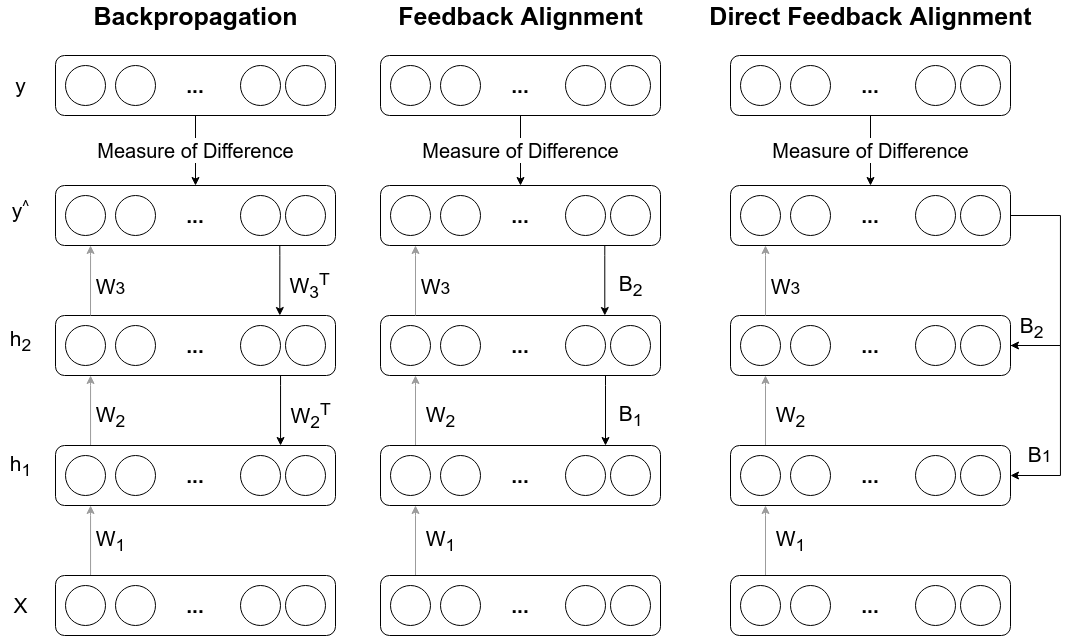
\includegraphics[width=1\linewidth]{figures/1_ErrorPropagation} 

}

\caption[Error Transportation in BP, FA, and DFA]{\textbf{Error Transportation in BP, FA, and DFA} \newline Visualization of the error transportation configurations for BP, FA, and DFA for two-layer networks \cite{nøkland2016direct}. $W_i$ are the weights, $h_i$ are the output of the hidden layers that is denoted as $i$, $\hat{y}$ is the output of the network, and $y$ is the ground truth, for the sake of simplicity, biases are not showed in this figure.}\label{fig:Error-Propagation}
\end{figure}

\noindent The figure \ref{fig:Error-Propagation} shows the difference in the algorithms' error propagation mechanisms that we mentioned before. In our experiments, we have used architecture with only one hidden layer, not the one in figure \ref{fig:Error-Propagation}. In that case, FA and DFA are identical because, with one layer, there is no room to propagate the random matrix in parallel.\\
It is crucial to point out, BP and DFA have different learning dynamics. BP calculates the gradients that point to the steepest descent in the loss function space. On the other hand, FA and DFA provide a different update direction but still descending. It is still descending because empirical and theoretical results proved that the networks' weights align with the random matrix that leads to gradients alignment. Therefore the more alignment we have, the same direction FA and DFA point as BP. However, it does not mean that more alignment is better performance because FA and DFA might find different and possibly better paths that converge to the global minimum. Even though they have different update directions, since they are both descending, the results from \cite{lillicrap2014random, nøkland2016direct} showed that FA and DFA are as good as BP in terms of performance for specified tasks in these papers. In addition to this, ANNs trained with DFA show decent separation for labels as in BP's hidden representations of the layers. It means that DFA captures similar information as BP.\\
Recently, a new study has been published which tests the applicability of DFA on modern deep learning tasks and architectures such as neural view synthesis, recommender systems, geometric learning, and natural language processing \cite{launay2020direct}. Because even though some of the alternative training algorithms that are competitive with BP in simple tasks like MNIST are not competitive or trainable on more complex tasks. This study showed that DFA successfully trains all these complex architectures with performance close to BP. Moreover, this study supports that complex tasks can be solved without symmetric weight transport, proving that DFA is suitable for more challenging problems.\\
Let us use the same example as \ref{chap:appendix_a} to present how gradients are calculated in DFA. After having the mathematical foundations of BP, transition to DFA is relatively easy. The forward pass is the same as BP, whereas, in the backward pass, we need to replace the transpose of the weight matrix, which is used to calculate the gradients with the random matrix. Considering the same example, we have a simple binary classification task with BCE loss, and our network has only one hidden layer. In this setting, gradients of the weights can be calculated as the following:
\[
\frac{\partial BCE}{\partial w_{2}}=h_{1}^T\left(\hat{y}-y\right)
\]
There is no change in the calculations of gradients of the last layer, whereas, for the hidden layer, we have:
\[
\begin{aligned}
\frac{\partial BCE}{\partial w_{1}}= \left(X\right)^T\left(\hat{y}-y\right)\left(B\right) \odot f'(a_1)
\end{aligned}
\]
Where \(y\) is the ground truth and \(\hat{y}\) is the output of the network, \(h_k\) is the output of the layer (which means that \(h_0 = X\) and \(h_2 = \hat{y}\)). \(a_{k} = h_{k-1} w_{k} + b_k\) where \(w_k\) is the weight, \(b_{k}\) is the bias term and f is the non linear function.
Please note that \(w_2^T\) is replaced with the random matrix \(B\). This means we can obtain learning by changing either the random matrix or weight matrix. We know that in DFA, \(B\) is fixed, so the feedforward weights of the network will learn to make these signals useful by aligning with the BP's teaching signal.\\
Update rules are the same as BP, which means gradient descent and its variants can be used. With this tiny modification, DFA brings a solution to some of the drawbacks of BP. Such as using exact symmetric weights of the feedforward connections (weight transport problem), lack of parallel processing (random matrix can be propagated in parallel), and it is less likely to suffer from vanishing or exploding gradients than BP. Eventually, it proposes a more biologically plausible training method. However, it is not the perfect solution either. Because it assumes there is a global feedback path to propagate the error that might be biologically implausible because feedback has to travel a long physical distance. It also suffers some of the drawbacks of BP. For instance, computation is still purely linear. We still need precise knowledge of derivatives of non-linearities. We still communicate by clean, continuous values, and it is unclear where the output targets would come from. Besides, DFA has an extra task to accomplish while training the ANN that aligns with BP's teaching signal, and a layer can not learn before its preceding layers are aligned. This might spawn performance concerns, and DFA might lag behind BP.
Furthermore, DFA fails to train convolutional neural networks which dominate the computer vision tasks \cite{refinetti2021align, launay2019principled}. Finally, unlike BP, DFA was not investigated on particular subjects like adversarial attacks and interpretability by the community. This leaves some question marks about the robustness of DFA.

\hypertarget{lazy-methods}{%
\section{Lazy Methods}\label{lazy-methods}}

Theoretical results present that especially over-parameterized ANNs (not limited to these networks) trained with gradient-based methods might reach zero training loss with their parameters barely changing (if they converge). The term lazy does not refer to the poor property of methods, whereas they are called lazy methods because their parameters hardly move during training \cite{chizat2020lazy}. This study uses the term lazy methods and linear methods interchangeably because the following algorithms show both properties. These properties are: essentially they are linear methods over a fixed representation of the data, and during the training phase, their parameters do not change too much (fixed representation).\\
Lazy methods are not at the center of our experiments. Hence, detailed explanations of these methods are out of scope in this study, but they have been presented in \cite{DBLP:journals/corr/abs-2002-07400, chizat2020implicit}, and they fail to learn the parities in a more complex setting. Also, they demonstrated poorer performance on the synthetic data problem. Given that, we will implement those methods too as a baseline and for completeness. We will also embody at least a simple definition of them and how they are practically implemented.\\
For this purpose, the following lazy methods will be explained: neural tangent kernel, gaussian features, reLU features, and linear features.

\hypertarget{neural-tangent-kernel}{%
\subsection{Neural Tangent Kernel}\label{neural-tangent-kernel}}

Studies showed that neural networks under some conditions are equivalent to a Gaussian process, and they mathematically approximate the kernel machines if they are trained with gradient descent \cite{lee2018deep, domingos2020model}. Authors of \cite{DBLP:journals/corr/abs-1806-07572} proved that during the training phase, ANNs follow the kernel gradient of the functional loss concerning a new kernel. They named this kernel a Neural Tangent Kernel (NTK). In other words, NTK is a kernel that describes the evolution of an ANN during the learning phase, and it is beneficial to explain the training of ANNs in function space rather than parameters space. It allows us to work with infinite width neural networks using the kernel trick, and it helps us understand the dynamics of learning and inference.\\
Empirical results demonstrated that the NTK regime performs worse than BP on standard tasks like MNIST. However, NTK is still worth investigating further to understand ANNs' training dynamics since it brings a new perspective on the training phase.\\
The practical implementation of NTK is obtained as the following: ``we used an architecture that decouples the gating from the linearity of the ReLU, and we kept the gates fixed during training. This means, by using \(\operatorname{ReLU}(\langle\mathbf{w}, \mathbf{x}\rangle)=\langle\mathbf{w}, \mathbf{x}\rangle \cdot \mathbf{1}\{\langle\mathbf{w}, \mathbf{x}\rangle\}\) and by decoupling the first and second term during the optimization, the network is forced to stay in NTK regime. \cite{DBLP:journals/corr/abs-2002-07400}'' In other words, an extra layer is created with the exact dimensions of the first layer. In the forward pass, concatenation of these two layers' parameters is given as input to the gated linear unit function. Lastly, the extra layer is not considered in the parameters update phase.

\hypertarget{random-features}{%
\subsection{Random features}\label{random-features}}

In standard random features, the first layer weights are initialized randomly by a distribution that we will specify in the following. The train is performed only for the second layer weights. In this way, the inputs are mapped into a fixed embedding space before a logistic separation. These mechanisms are particularly good at approximating kernels. They are preferred over kernels because the latter might take too much time to train if the data size is big. In \textbf{gaussian features} case, we initialize the first layer weights using a gaussian distribution. In \textbf{ReLU features} and \textbf{linear features}, we initialize the first layer weights by a uniform distribution. The distinction of the last two regimes is that in the forward pass, non-linear activation functions are replaced by linear ones for linear features.

\hypertarget{optimizers}{%
\section{Optimizers}\label{optimizers}}

Up to this point, we only mentioned how we could use gradient descent and its variants to update the weights of a network superficially. This part is worth further investigation because many variants provide better convergence properties to find the minimum of the loss function. We may take advantage of these methods to have better performance or faster convergence for BP and DFA. These methods may spawn a significant impact on convergence speed and overall performance. As a reference to the following methods, mostly \cite{DBLP:journals/corr/Ruder16} is used, also the structure of this part and mathematical notations are adapted from the same paper, it is an excellent overview for the optimizers, and it reviews their advantages as well as drawbacks.

\hypertarget{gradient-descent}{%
\subsection{Gradient Descent}\label{gradient-descent}}

Gradient descent is a first-order iterative optimization algorithm. It is the most used algorithm to optimize neural networks. It has three variants that depend on how much data we use to compute the gradients. \textbf{Batch gradient descent} computes the gradients for the entire dataset and performs only one update. \textbf{Stochastic gradient descent} (SGD), in contrast, calculates gradients for each training example and performs parameter update for each of them. Lastly, \textbf{mini-batch gradient descent} calculates the gradients of mini-batches and performs updates for each mini-batches.
Gradient descent is infeasible for the datasets that do not fit in the memory. In contrast, SGD performs too frequent updates, spawning high variance in parameters that cause fluctuation in the loss function. SGD provides the same convergence properties as batch gradient descent if the learning rate periodically decreases through iterations. We used mini-batch gradient descent for our experiments, which takes the best of two methods. Most of the implementations use SGD term instead of mini-batch gradient descent. The same tradition will be followed in this study too. Update rule of mini-batch gradient descent is the following:
\[
\theta_{t+1}=\theta_t-\eta \cdot \nabla_{\theta} J\left(\theta ; x^{(i: i+n)} ; y^{(i: i+n)}\right)
\]
where \(\theta\) is the parameters of the network, \(\eta\) is the learning rate or step size, \(\nabla_{\theta}\) is the gradients of the parameters and \(J\left(\theta ; x^{(i: i+n)} ; y^{(i: i+n)}\right)\) is the loss function for mini-batch \(i\) to \(i+n\).\\
There are a couple of challenges in SGD because it doesn't always guarantee good convergence:

\begin{itemize}
  \item Choosing a proper learning rate is intricate. Low learning rates may take too long to converge, whereas big learning rates may spawn loss function fluctuations and even diverge.
  \item SGD does not guarantee the global minimum. It can easily be stuck in the local minimum for highly non-convex loss functions standard for deep learning tasks.
  \item Same learning rate is applied to all parameters, but we may want to update the parameter by their frequencies.
  \item Convergence is strongly dependent on where the initial step starts. Unfortunate initializations may never reach the global minimum. 
\end{itemize}

\hypertarget{momentum}{%
\subsubsection{Momentum}\label{momentum}}

\noindent SGD has difficulties finding the direction in valleys because the gradients on these areas will be either zero or very close to zero, so it will slow down and make hesitant progress. These areas are prevalent around the local minimum. Momentum is an idea that dampens the oscillations in the relevant direction. It is accomplished by adding a fraction \(\gamma\) of the update vector of the past time step. This fraction is usually set to \(0.9\). This term usually leads to faster convergence and speeds up the iterations.
\[
\begin{aligned}
v_{t} &=\gamma v_{t-1}+\eta \nabla_{\theta} J(\theta) \\
\theta_{t+1} &=\theta_t-v_{t}
\end{aligned}
\]
However, momentum follows the direction of the gradients blindly, \textbf{nesterov accelerated gradient} (NAG) is a way of giving our method to intuition by approximating the next position of the parameters with \(\theta -\gamma v_{t-1}\), with this we hope to slow down before the hill slopes up. In other words, first, as in the momentum method, we make a big jump in the direction of previous gradients, then we measure the gradients where we end up and make a correction. The new update rule becomes:
\[
\begin{aligned} v_{t} &=\gamma v_{t-1}+\eta \nabla_{\theta} J\left(\theta-\gamma v_{t-1}\right) \\ 
\theta_{t+1} &=\theta_t-v_{t} \end{aligned}
\]

\hypertarget{adaptive-methods}{%
\subsection{Adaptive Methods}\label{adaptive-methods}}

Two main drawbacks of SGD are: tuning the learning rate is complex, and we use the same learning rate for each parameter. Adaptive methods offer solutions to these problems. They use intelligent ways to modify the learning rate that may differ from parameter to parameter, and some of them even remove the need to set the learning rate. However, they are still gradient-based algorithms with some modifications, and they do not always guarantee convergence.

\hypertarget{adagrad}{%
\subsubsection{Adagrad}\label{adagrad}}

\noindent In vanilla SGD and SGD with momentum, we used the same learning rate for each parameter. On the contrary, adagrad adapts the learning rates for each parameter. It performs larger updates for infrequent features and smaller updates for frequent features. By saying infrequent features, we mean the cases where the component of the feature has a value different than the most common one. Usually, this component is important and informative. These values are called infrequent features. To do this, it updates the learning rate at each time step \(t\) for each parameter based on their past gradients concerning the loss function.
\[
\theta_{t+1}=\theta_{t}-\frac{\eta}{\sqrt{G_{t}+\epsilon}} \odot g_{t}
\]
With this update rule, the learning rate is modified at each time step. \(G_t\) contains the sum of squares of the past gradients for all parameters. \(g_t\) is the gradients of all parameters at time step \(t\), and \(\epsilon\) is the smoothing constant to avoid zero division, and it is usually set to \(10^{-8}\). \(G_t\) is getting larger with each step since we only add positive terms that make the learning rate very small, and the algorithm cannot learn any more in advancing time steps.

\hypertarget{adadelta}{%
\subsubsection{Adadelta}\label{adadelta}}

\noindent Adadelta is an extension of Adagrad, which tries to solve the decreasing learning rate problem and tries to remove the need for tuning the learning rate manually \cite{zeiler2012adadelta}. Instead of using the squares of all past gradients, Adadelta sets a moving window of gradient updates, and by doing so, it continues learning even after many iterations. It does by storing the exponentially decaying average of the squared gradients.
\[
E\left[g^{2}\right]_{t}=\rho E\left[g^{2}\right]_{t-1}+(1-\rho) g_{t}^{2}
\]
\(E\left[g^{2}\right]_{t}\) is the running average, \(\rho\) is the decay constant which is similar to momentum term (it is usually set to around \(0.9\) like momentum). The demonitor of the update rule of adadelta is very similar to adagrad, only difference is \(G_{t}\) is replaced with \(E\left[g^{2}\right]_{t}\). The term \(\sqrt{E\left[g^{2}\right]_{t}+\epsilon}\) can be rephrased as root mean squares of the previous gradients up to time \(t\).
\[
\operatorname{RMS}[g]_{t}=\sqrt{E\left[g^{2}\right]_{t}+\epsilon}
\]
Where \(\epsilon\) is a smoothing constant for avoiding any problem in the denominator, by using this term, we can change the update rule of Adagrad to the following:
\[
\theta_{t+1}=\theta_{t}-\frac{\eta}{R M S[g]_{t}} \odot g_{t}
\]
For clarity, we can rephrase the update rule as follows:
\[
\theta_{t+1} = \theta_{t} + \Delta \theta_{t} \\
\]
where;
\[\Delta \theta_{t} = -\frac{\eta}{R M S[g]_{t}} \odot g_{t}\]
Authors of \cite{zeiler2012adadelta} pointed out that parameters updates in SGD, momentum and Adagrad doesn't match with the units of the parameters. The units relate the gradients, not the parameters. To overcome this issue they defined exponentially decaying average of parameters instead of gradients.
\[
E\left[\Delta \theta^{2}\right]_{t}=\rho E\left[\Delta \theta^{2}\right]_{t-1}+(1-\rho) \Delta \theta_{t}^{2}
\]
The root means squared error of the parameters is:
\[
\operatorname{RMS}[\Delta \theta]_{t}=\sqrt{E\left[\Delta \theta^{2}\right]_{t}+\epsilon}
\]
Since \(\operatorname{RMS}[\Delta \theta]_{t}\) is unknown at time step \(t\), it is approximated with previous time step.
\[
\theta_{t+1}=\theta_{t} - \frac{R M S[\Delta \theta]_{t-1}}{R M S[g]_{t}} g_{t}
\]
Normally this final update would remove the need for a learning rate. However, we follow the same approach as in Pytorch implementation \cite{NEURIPS2019_9015} so the last term is scaled with learning rate, which finally yields to update rule of Adadelta:
\[
\theta_{t+1}=\theta_{t} - \eta \frac{R M S[\Delta \theta]_{t-1}}{R M S[g]_{t}} g_{t}
\]

\hypertarget{rmsprop}{%
\subsubsection{RMSProp}\label{rmsprop}}

\noindent RMSProp is another method offered to solve the decreasing learning rate problem of adagrad. Geoffrey Hinton proposed it in his neural networks for machine learning class\footnote{\url{http://www.cs.toronto.edu/~tijmen/csc321/slides/lecture_slides_lec6.pdf}}. It is identical to the first update rule of Adadelta that is:
\[
\begin{aligned}
E\left[g^{2}\right]_{t}=\rho E\left[g^{2}\right]_{t-1}+(1-\rho) g_{t}^{2} \\
\theta_{t+1}=\theta_{t}-\frac{\eta}{\sqrt{E\left[g^{2}\right]_{t}+\epsilon}} \odot g_{t}
\end{aligned}
\]
Similar to momentum constant, it is suggested to set \(\rho\) to \(0.9\), and \(\epsilon\) is the smoothing constant similar to previous methods' update rules.

\hypertarget{adam}{%
\subsubsection{ADAM}\label{adam}}

\noindent Adam is another adaptive method that adjusts the learning rates for each parameter. It also stores an exponentially decaying average of past and squared gradients similar to momentum. It combines the best properties of adagrad and RMSProp algorithms.
\[
\begin{aligned}
m_{t} &=\beta_{1} m_{t-1}+\left(1-\beta_{1}\right) g_{t} \\
v_{t} &=\beta_{2} v_{t-1}+\left(1-\beta_{2}\right) g_{t}^{2}
\end{aligned}
\]
Where \(m_t\) is the estimate of the first moment of the gradients and \(v_t\) is the estimate of the second moment. However, the authors noticed that these two terms are biased towards zero with zero initialization. Therefore they proposed bias-corrected forms of these terms to overcome this problem. It is suggested to set default values for \(\beta_1\) and \(\beta_2\) as \(0.9\) and \(0.999\).

\[
\begin{aligned}
\hat{m}_{t} &=\frac{m_{t}}{1-\beta_{1}^{t}} \\
\hat{v}_{t} &=\frac{v_{t}}{1-\beta_{2}^{t}}
\end{aligned}
\]
Then the update rule is very similar to Adadelta and RMSProp that is:
\[
\theta_{t+1}=\theta_{t}-\frac{\eta}{\sqrt{\hat{v}_{t}}+\epsilon} \hat{m}_{t}
\]

\hypertarget{t-sne}{%
\section{t-SNE}\label{t-sne}}

t-distributed stochastic neighbor embedding (t-SNE) is a method visualizing high-dimensional data which tries to keep the neighbor property in lower dimensions \cite{vanDerMaaten2008}. It is an unsupervised, non-linear dimensionality reduction technique commonly used for visualization purposes. It is beneficial to understand how data is structured in a high-dimensional space.\\
The idea of the algorithm is the following: first, it calculates the similarity between pairs in the high dimensional space and the low dimensional space. Then it tries to minimize these two similarity measures. The similarity measures are calculated by converting high-dimensional Euclidean distance to conditional probabilities. Each point centered a Gaussian distribution. This probability will be relatively high for closer points, whereas, for farther points, it will be smaller. For low-dimensional counterparts, a similar process can be followed. However, unlike stochastic neighbor embedding, \cite{Hinton_Roweis_2003}, student t-distribution with one degree of freedom (Cauchy distribution) is employed instead of Gaussian distribution. It is a heavy-tailed distribution that helps map the points far apart in low-dimensional space. After having two similarity measures, the objective is minimizing the mismatch among them. The objective function is expressed using Kullback-Leibler divergences and is optimized using a gradient descent method.\\

\noindent \textbf{Highlights}\\
\noindent With t-SNE, we completed the theoretical overview of the methods used for the experiments. We started with the simple definition of BP. We explained how the error is propagated in BP and how gradients are calculated mathematically. We also mentioned the drawbacks of BP. Then, we moved to DFA by slightly changing the error propagation mechanism of BP, and we adapted this change to our mathematical foundations. We specified which drawbacks of BP were addressed by DFA, and we also mentioned the limitations of DFA. After that, lazy methods are summarized since they are implemented and used in experiments of previous studies. Then, optimizers are described in general. We mentioned why they are essential and how they might increase the convergence property, and we presented their update rules and drawbacks. Lastly, the idea of t-SNE is explained superficially.

\hypertarget{chap:chapter_2}{%
\chapter{Learning Problems}\label{chap:chapter_2}}

\minitoc 

\noindent The success of neural networks spawned a great interest in comparing the predictive power of the various models. This involves testing different models on the same learning problem, usually difficult to learn, and observing which model performs better. It is particularly beneficial to understand their learning dynamics, which helps discover their limitations. These studies achieved striking success in finding out the superiority of the neural networks over linear methods. Given that, we are curious about the place of the DFA on these problems. For this purpose, we consider two learning problems: \textbf{parity learning} and \textbf{synthetic data problem}.

\hypertarget{parity-learning-problem}{%
\section{Parity Learning Problem}\label{parity-learning-problem}}

The parities are notoriously hard to learn by ANNs \cite{DBLP:journals/corr/abs-1807-06399}. By taking advantage of this situation, in \cite{DBLP:journals/corr/abs-2002-07400}, authors questioned how far neural networks could go beyond the linear models. They did this by focusing on parities that have a complex family of target functions. They demonstrated that this family could be approximated by a two-layer network trained with Adadelta but not by lazy methods. This study brings an explanation of why neural networks' performance is better than linear methods, and it proves neural networks' learning capacities are beyond them.\\
Experiments are performed on the MNIST dataset by imitating the parity problem. The task is: given a parameter k (defines the number of digits to be stacked together that is chosen uniformly from the dataset), determine if the sum of the digits is odd or even. When \(k=1\), it is a simplified version of the standard MNIST task to find if a digit is even or odd. Experiment results showed that all models, including the lazy ones, reached a similar performance in the \(k=1\) case where the neural network slightly outperformed others. On the other hand, the problem becomes more difficult for the case \(k=3\) because models need to compute the parity of the digits' sum. In this case, there is a drastic gap between the neural network and lazy methods. Because the predictions of lazy methods did not go beyond the random guess.\\
Since our goal is comparing DFA and BP on this particular problem, reproducing the results from \cite{DBLP:journals/corr/abs-2002-07400} is unavoidable. The same configurations are used with minor differences and, they are implemented in Pytorch \cite{NEURIPS2019_9015}. The network has only a hidden layer with \(512\) neurons. For the last layer, sigmoid is used as a non-linear activation function. For the hidden layer, reLU is used. BCE is preferred as a loss function, and we have not used weight decay. In addition to previous settings, we have also used SGD to observe how much Adadelta improves. For the case \(k=3\), we performed a simple hyper-parameter tuning process to get a decent learning rate for each method. Same learning rate values are used for the case \(k=1\). The hyperparameter tuning process is the following. First, we define the parameter space, later we run with all different learning rates, and we compare these runs by the average of test accuracy of the last ten epochs, and we choose the highest one. It is also crucial to mention that, at each epoch, train data is recreated to boost the available data for the models. The same is also performed for test data to have an unbiased estimation of test accuracy. It implicitly prevents overfitting and increases the available data because the data creation is stochastic. The process is the following: random images are sampled uniformly from the available dataset, then according to given parameter \(k\), these random images are horizontally stacked. Hence we have different dataset at each epoch that helps networks to learn and perform better. Finally, these images are normalized before training the networks, which is necessary for deep learning tasks.

\begin{figure}

{\centering 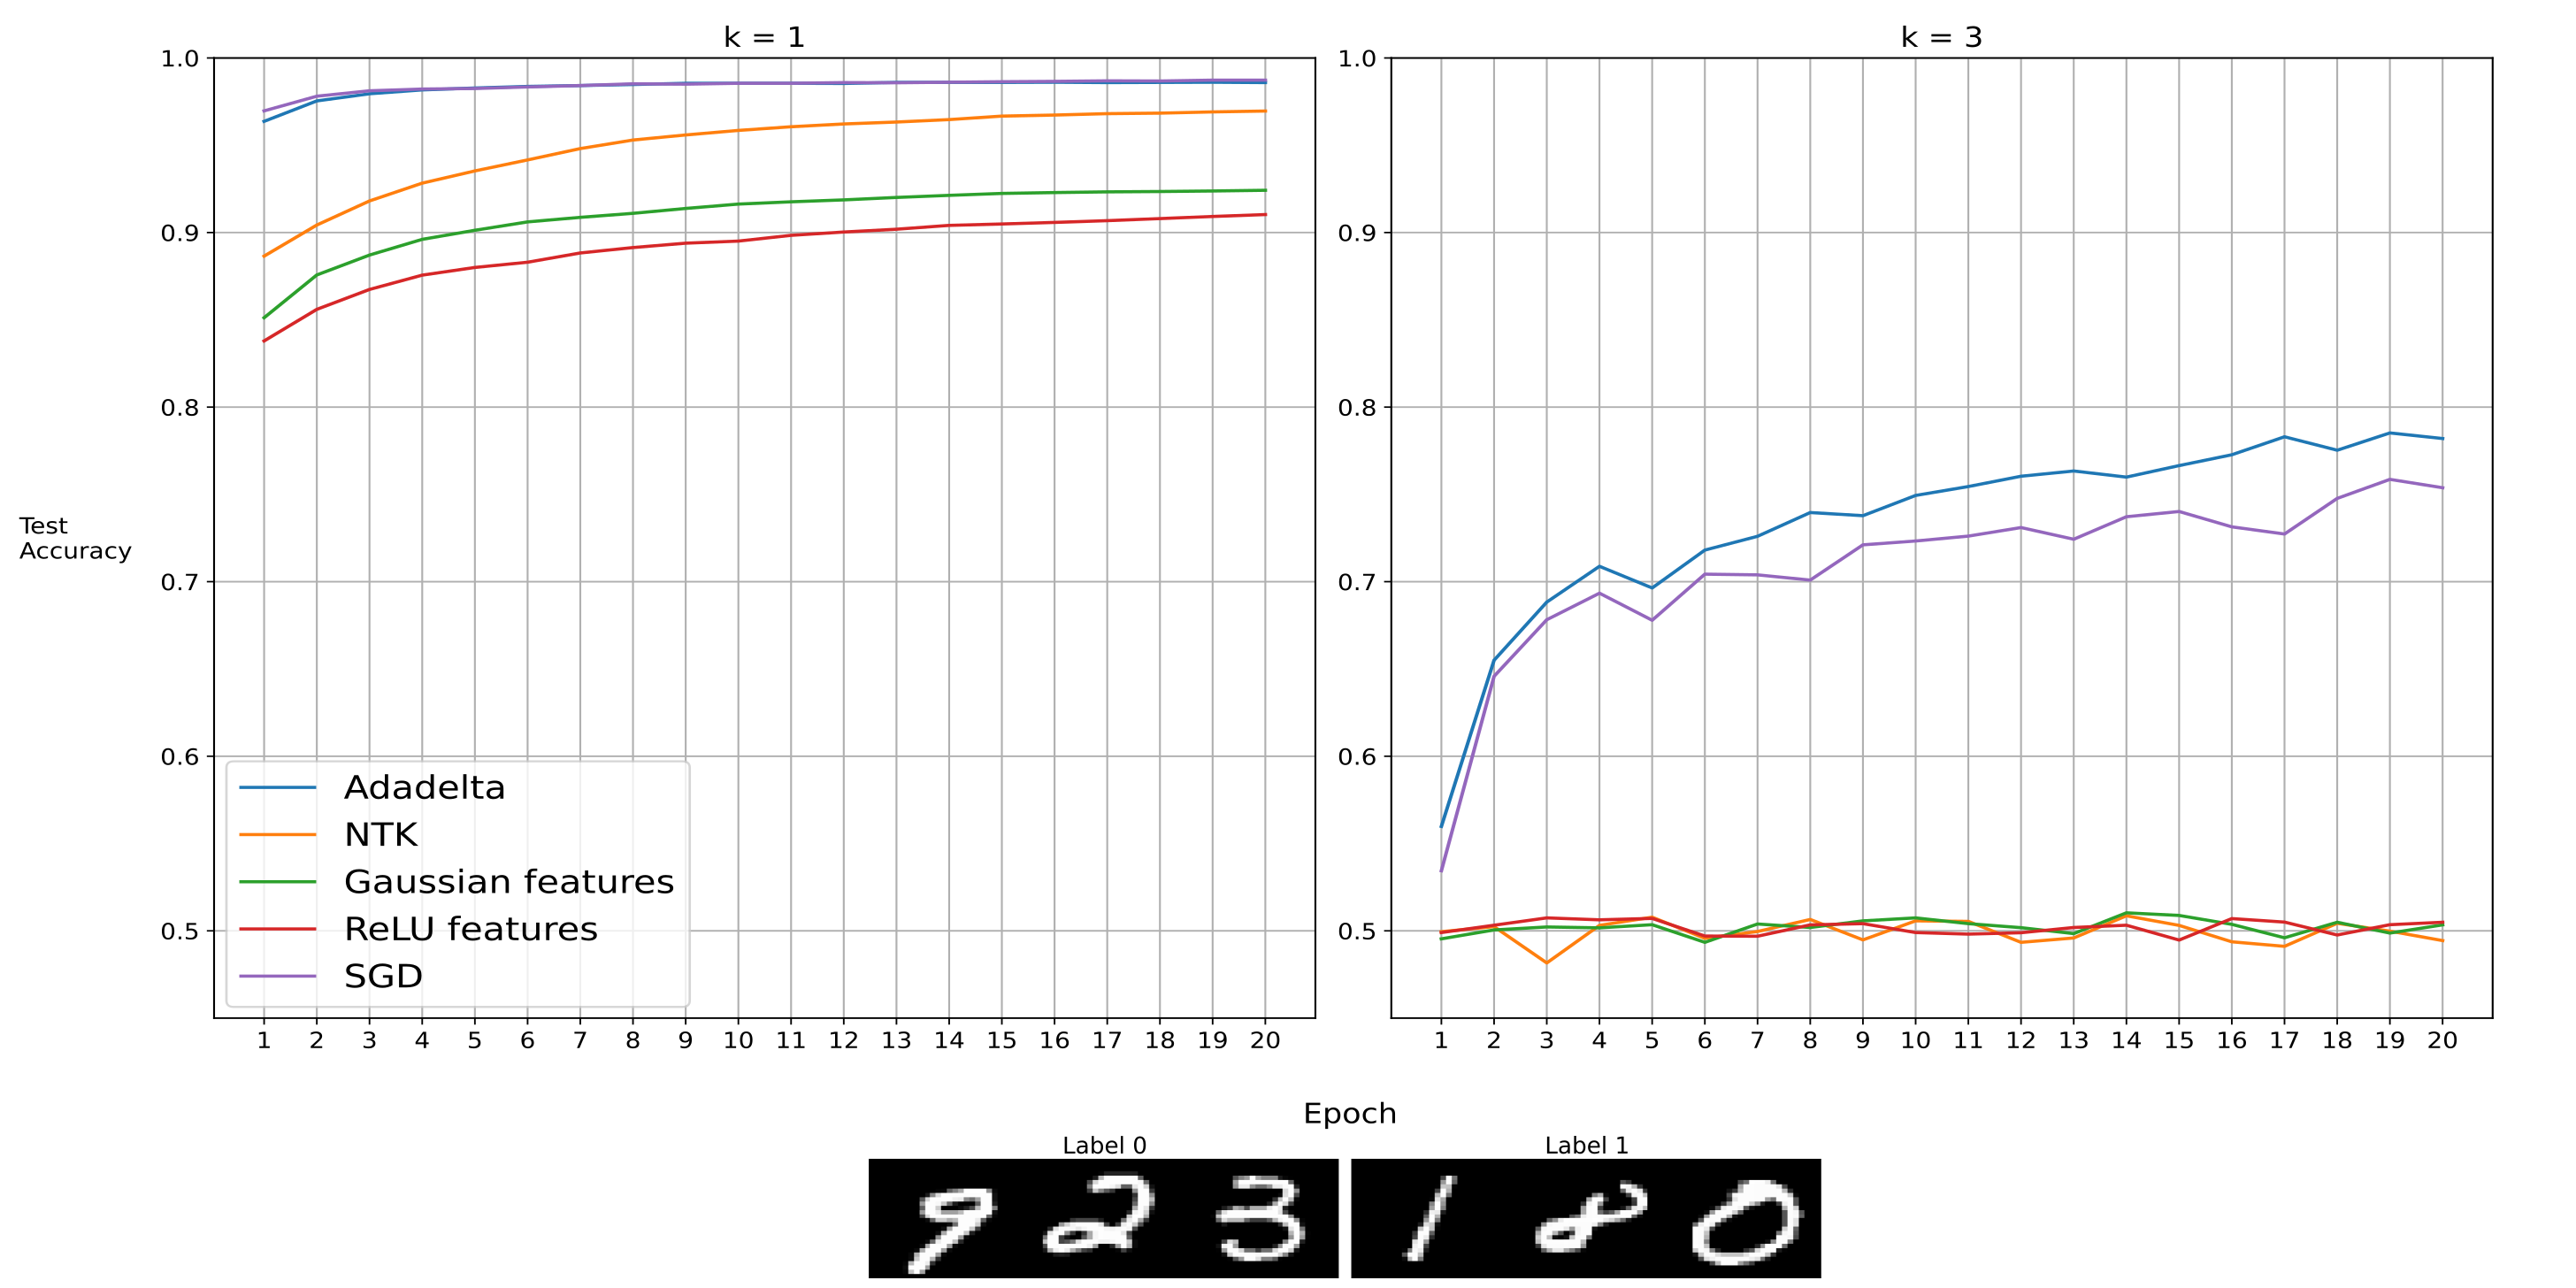
\includegraphics[width=1\linewidth]{figures/2_k13_SGD_ada_BP_reproduced} 

}

\caption[Reproduced MNIST-Parity Experiment]{\textbf{Reproduced MNIST-Parity Experiment} \newline Reproduced MNIST-Parity experiment from \cite{DBLP:journals/corr/abs-2002-07400}. The top left is the test accuracy for the parity of a single image. The top right is the test accuracy for parity of three images. The bottom is the examples from the dataset. The model needs to predict the parity of the sum of the digits.}\label{fig:MNISTparity}
\end{figure}

\noindent The reproduced result can be observed in figure \ref{fig:MNISTparity}. Similar to results from \cite{DBLP:journals/corr/abs-2002-07400}, all the methods succeed learning for \(k=1\) case. However, adadelta and SGD slightly outperformed lazy methods in this setting. In the case of \(k=3\), adadelta and SGD almost reach \(80\%\), but the performance of lazy methods does not go beyond a random guess.~
After having the concrete picture from the previous study, it is intriguing to see how DFA would perform with SGD and adaptive methods on this particular problem. We will investigate it in chapter \ref{chap:chapter_3} with other experiments.

\hypertarget{synthetic-data-problem}{%
\section{Synthetic Data Problem}\label{synthetic-data-problem}}

In \cite{chizat2020implicit}, the authors presented implicit bias in two-layer neural networks with cross-entropy loss trained with SGD. Implicit bias is a phenomenon that indicates that SGD is not only successful in finding the global minimum but also is biased towards solutions that generalize well \cite{yun2021unifying}. The study is beneficial to observe this phenomenon of gradient methods and training dynamics of wide neural networks. After demonstrating theoretical results, they performed numerical experiments to validate these results. The numerical experiments have a binary classification problem, and the data are synthetically generated. The problem is an example of a task where the inputs have a lower-dimensional structure. The number of samples and dimensions can be adjusted in the dataset. Similar to parity experiments, the results demonstrated the superiority of the neural network to the lazy method. Considering that all the nice properties of the dataset and the similarity of our previous comparison, it is an excellent problem to compare BP and DFA. Besides, it is nicer to compare BP and DFA in another challenging learning problem which the difficulty of it can be adjusted to avoid limiting our experiments with only the MNIST-Parity task.\\
\noindent Given the parameter \(c\) that denotes the number of clusters (in \cite{chizat2020implicit}, this parameter is denoted as \(k\) since we used the same notation in parity problem, to avoid any confusion it is changed). The data is generated as the following: in dimension \(d=2\), the distribution of the input values is a mixture of \(c^2\) uniform distributions on the disk of radius \(1/ (3c-1)\) on a uniform two-dimensional grid with step \(3/(3c-1)\). Larger dimensions follow the uniform distribution on \([-1/2,1/2]\). Each cluster is assigned randomly to a label \cite{chizat2020implicit}. In other words, after having the cluster centers, each input is sampled by following the uniform distribution with the shift angle and magnitude for dimension \(2\). Each input value is sampled from a uniform distribution for other spurious dimensions. Unlike the paper, labels are \(0,1\), not \(-1,1\) because it fits the structure of our previous architecture and training mechanism used for the parity experiment.\\
Like the parity problem, before testing DFA on the problem, it is beneficial to reproduce results from the previous study. For this purpose, the scratch implementation is used with the same architecture (only a hidden layer, \(512\) layer size, with reLU and sigmoid non-linearities). For each \(n\) (number of training samples) and \(d\) (number of dimensions, \(\geq2\)), experiments were performed three times, and they are plotted with a \(95\%\) confidence interval. Similar to the paper, the learning rate is set to \(0.5\) (no hyperparameter tuning process is performed for this problem), weight decay is not used, and the epoch number is \(500\). We give enough time for all methods to converge with this high epoch number.

\begin{figure}

{\centering 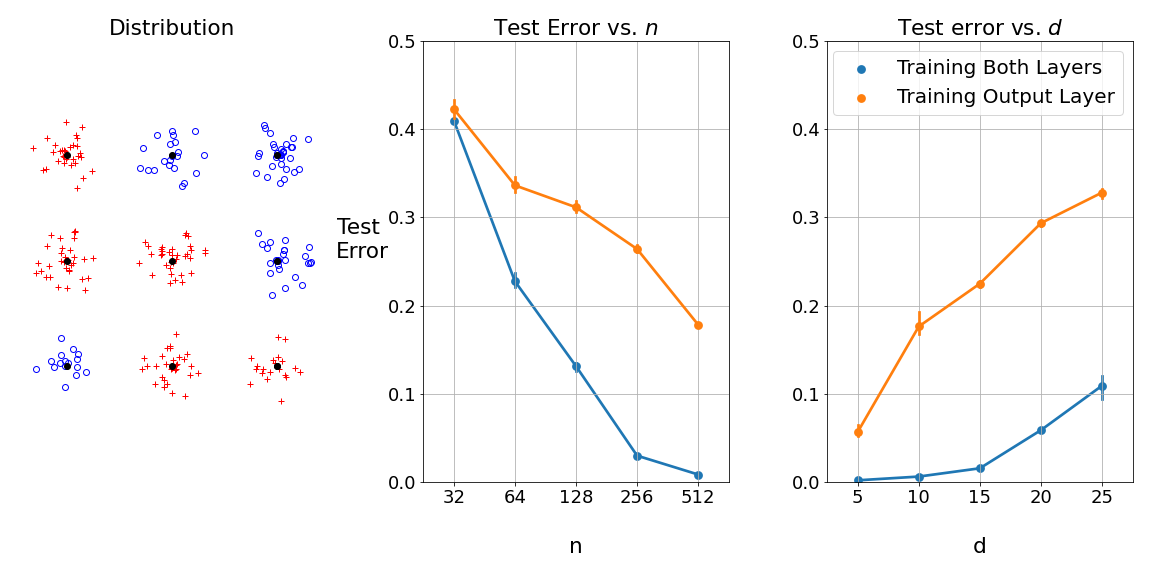
\includegraphics[width=1\linewidth]{figures/2_syntheticData_reproduced} 

}

\caption[Reproduced Synthetic Data Experiment]{\textbf{Reproduced Synthetic Data Experiment} \newline Reproduced synthetic data experiment from \cite{chizat2020implicit}. The networks are trained with backpropagation and SGD. On the left, distribution of the input on two first dimensions. In the middle, test error as a function of the number of inputs ($n$) with $d=15$. On the right, test error as a function of the number of dimensions ($d$) with $n=256$.}\label{fig:randomData}
\end{figure}

\noindent We can observe the reproduced experiment results in figure \ref{fig:randomData} from \cite{chizat2020implicit}. We have the data distribution in two-dimension on the left with \(c=3\) (so we have 9 clusters) used for the experiment. This distribution is chosen because it is difficult to learn (it is not linearly separable). We have the test error and an increasing number of training samples in the middle plot where the dimension is \(15\). We expect to observe decreasing test error with the increasing number of training samples for each model. On the right, we have the test error and the number of dimensions where the number of samples is \(256\). The problem becomes challenging with the increasing number of dimensions because extracting useful information becomes more difficult for models with higher dimensional input since they are non-informative. Therefore we see the increasing test error. Similar to the paper results, we observe that training both layers gives better results than training only the output layer. In other words, increasing the number of training samples helps more to network than the lazy method, and the neural network is more successful in distinguishing useful inputs in high dimensions for this problem. It is important to mention that we have used only one distribution with \(3\) repetition. The result may vary on distribution but on average; we should observe the superiority of BP as it is presented in \cite{chizat2020implicit}. It is interesting to put DFA in this frame to observe if it is closer to the lazy method or BP.\\

\noindent \textbf{Highlights}\\
After having the reproduced results for the synthetic data problem, we completed the chapter on learning problems. First, we explained the problems and described how their data were generated and the task. Then we explained the details of the architectures of the networks, hyperparameter tuning process, and training phase used in the experiments. We presented the reproduced results from the papers and motivated the testing DFA on these problems.

\hypertarget{chap:chapter_3}{%
\chapter{Experiments}\label{chap:chapter_3}}

\noindent After having the previous study results, we can continue to test DFA on the learning problems. Train phase and the hyperparameter tuning process are explained in chapter \ref{chap:chapter_2}. These processes are the same for the following experiments. For all experiments, scratch implementations are used with minimal Pytorch functionalities. They are performed three times and plotted with their confidence interval.\\
The same architectures are used as the previous studies for BP and DFA, meaning that we have only a hidden layer with 512 neurons for both problems, and reLU is used as a non-linear function for the hidden layer. BCE is chosen as a loss function and, sigmoid is preferred for the non-linearity of the last layer. For the parity problem, networks are trained for 20 epochs unless others are specified, and at each epoch, train and test datasets are recreated as it is explained in chapter \ref{chap:chapter_2}. For the synthetic data problem, networks are trained for 500 epochs. Weights of the networks are initialized uniformly with \(\frac{1}{\sqrt{input dim}}\) as in default Pytorch weight initialization. Moreover, the random matrix \(B\) is initialized with the same way to have similar behaviors as the weight matrix unless other specified.

\hypertarget{parity-learning-experiments}{%
\section{Parity Learning Experiments}\label{parity-learning-experiments}}

For each experiment, when there is a change in the training method (DFA or BP) or optimization method, hyperparameter tuning is performed to obtain a decent learning rate. Weight decay is not used for the experiments. Since the experiment details are precise, we can test DFA on the parity learning problem with BP using SGD.

\begin{figure}

{\centering 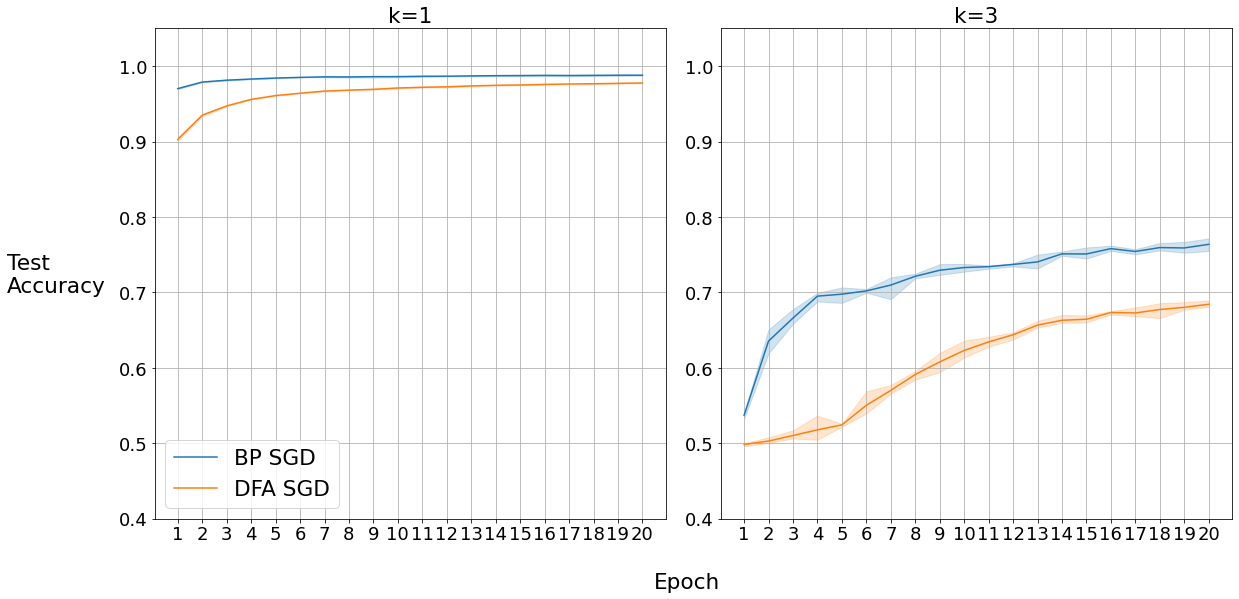
\includegraphics[width=1\linewidth]{figures/3_k13_SGD_DFAvsBP} 

}

\caption[BP and DFA on MNIST-Parity Problem with SGD]{ \textbf{BP and DFA on MNIST-Parity Problem with SGD} \newline The predictive power of DFA is presented on the MNIST-Parity experiment among BP. The left is the test accuracy for the parity of a single image. The right is the test accuracy for the parity of three images.}\label{fig:BPvsDFA}
\end{figure}

\noindent We can observe the results in \ref{fig:BPvsDFA} with \(95\%\) confidence interval. In the case \(k=1\), although DFA outperforms the lazy methods, it is behind the BP. In the case \(k=3\), it is obvious that DFA performs much better than lazy methods. However, the gap between BP and DFA is a bit higher than the \(k=1\) case. It seems like there is a limit for DFA to reach with SGD that is around \(\%70\). The reason is that DFA has an additional task to accomplish, which is aligning with BP's teaching signals. In other words, the network loses time while making teaching signals useful. This delays the convergence and causes performance lag. We can see that during the first iterations, DFA does not converge fast enough to catch up with BP, and it always stays behind it.\\
The thrilling question is, is there a performance limit for DFA to reach, and can we get a similar performance as BP by making some changes? For answering the first question, it is better to run DFA for more epochs to see if it can reach a similar performance as BP. Because with longer training, DFA will have time to align and converge. It would be convenient to test DFA with different random matrices to observe any improvement for the second question. Because it is clear that learning in DFA is strongly dependent on random matrix. Besides, it is interesting to test if DFA can learn with different random matrices. While tuning the learning rate for DFA, we noticed that it is susceptible to the learning rate. Low learning rates caused no convergence, and larger learning rates showed over-fitting within specified epoch numbers. Therefore we can use adaptive methods to have better convergence properties in BP and DFA. These methods are specifically good at adjusting the learning rate, which is more difficult to tune for DFA than BP.\\
\noindent We trained DFA for 50 epochs with a tuned learning rate to observe if it can reach a similar performance as BP. At the same time, alignment between the random matrix and the transpose of the weight matrix is plotted. This alignment is measured by using the cosine similarity.

\begin{figure}

{\centering 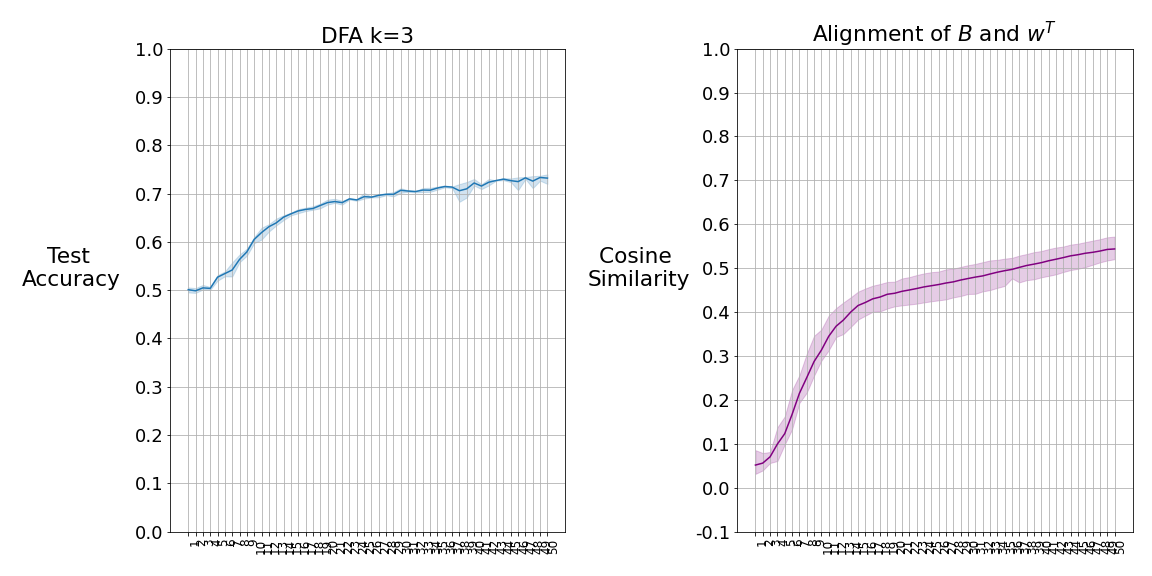
\includegraphics[width=1\linewidth]{figures/3_k3_SGD_DFA_Alingment} 

}

\caption[DFA on MNIST-Parity Problem with Alignment]{\textbf{DFA on MNIST-Parity Problem with Alignment} \newline DFA on MNIST-Parity task for the case $k=3$ trained $50$ epochs. The left is the test accuracy of DFA, and the right is the cosine similarity of the random matrix and the transpose of the weight matrix.}\label{fig:DFA50epochs}
\end{figure}

\noindent From figure \ref{fig:DFA50epochs}, we can see that DFA can reach a similar performance as BP trained with SGD. This result approves our comments about the additional task DFA has and why it takes longer to achieve the same performance. On the right side of the plot, we can examine the alignment between the random matrix and the transpose of the weight matrix. At the beginning of training, the similarity is low. However, we can see that alignment increases, similar to the performance with advancing steps. It shows that the network aligns with the BP's teaching signals. In other words, the network learns how to learn by using the random matrix.
\noindent After having a similar performance from DFA with SGD, it is intriguing to test if we can achieve similar performance within the same epoch number. For this purpose, the first improvement attempt will be related to random matrices. Using different random matrices may influence the performance of DFA. Some of them might align better with BP's teaching signals. On the other hand, it is interesting to observe if we can learn with any random matrix.\\
Apart from uniform random matrix, three different random matrices are tested. They are initialized as the following: \textbf{standard uniform} is default Pytorch initialization that is uniformly distributed from \(0\) to \(1\). \textbf{Gaussian} is initialized normally with \(\mu\) and \(\sigma\) are equal to each other that is \(\frac{1}{\sqrt{input dim}}\). Lastly, \textbf{standard gaussian} is initialized with \(\mu=0\) and \(\sigma=1\).

\begin{figure}

{\centering 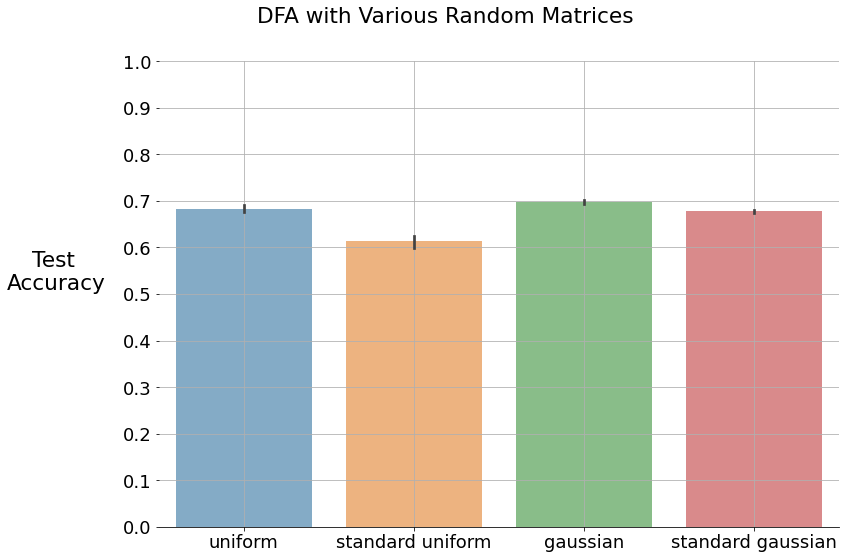
\includegraphics[width=1\linewidth]{figures/3_k3_DFA_RandomMatrices} 

}

\caption[DFA on MNIST-Parity Problem with Various Random Matrices]{\textbf{DFA on Parity Problem with Various Random Matrices} \newline The final test accuracy of DFA on the MNIST-Parity for the case $k=3$. The experiments performed three times and plotted with $95\%$ confidence interval. The random matrices are initialized as the following: $\text{standard uniform} \sim U(0,1)$, $\text{uniform} \sim U(-a,+a)$, $\text{standard gaussian} \sim \mathcal{N}\left(0, 1\right)$ and $\text{gaussian} \sim \mathcal{N}\left(a, a \right)$ where $a= \frac{1}{\sqrt{input dim}}$.}\label{fig:DFARandomMatrices}
\end{figure}

\noindent From figure \ref{fig:DFARandomMatrices}, we can observe that DFA can learn with any random matrices. However, it is essential to specify that learning rates for each random matrix are tuned and drastically different. Apart from standard uniform, the rest of the random matrices achieved similar performances, but they are still behind the BP. However, thanks to these results, we can see that DFA is highly sensitive to the learning rate. Because during the tuning phase, small learning rates did not converge within the specified epoch number. On the other hand, high learning rates demonstrated overfitting for each random matrices. Therefore, since adaptive methods have better convergence properties, they may increase the performance of DFA as they did in BP. For the rest of the DFA experiments, the random matrix is uniformly initialized since there is no significant improvement with other initializations.\\
\noindent Following the previous deduction, various adaptive methods are tested on the parity learning problem for BP and DFA. Their learning rates are tuned, as explained in the previous chapter. For the experiments, they are run three times, and their final test accuracies are plotted. The results are presented in figure \ref{fig:mainExperiment}.

\begin{figure}

{\centering 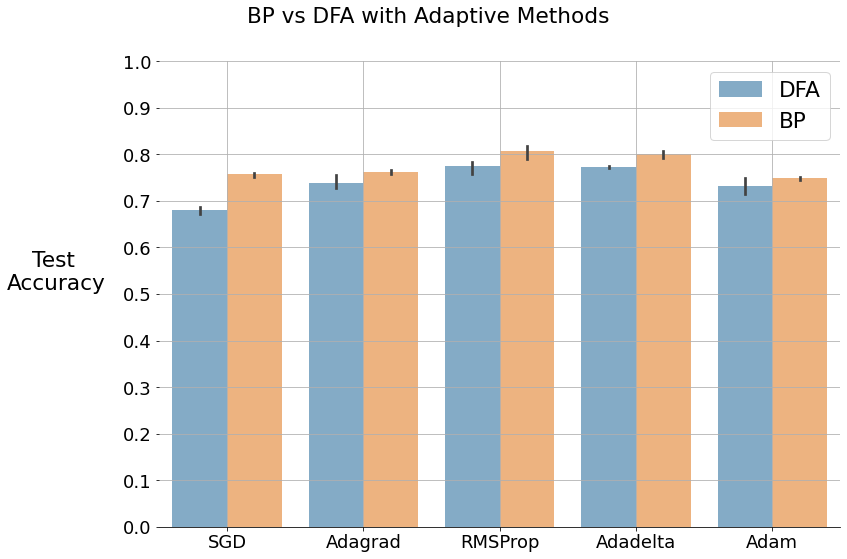
\includegraphics[width=1\linewidth]{figures/3_mainExperiment} 

}

\caption[DFA and BP on MNIST-Parity Problem with Adaptive Methods]{\textbf{DFA and BP on MNIST-Parity Problem with Adaptive Methods} \newline The final test accuracies are presented for BP and DFA with adaptive optimization algorithms. The experiments were performed three times and plotted with a $95\%$ confidence interval.}\label{fig:mainExperiment}
\end{figure}

\noindent As expected, adaptive methods improve the final test accuracy significantly for both BP and DFA. On average, DFA is still behind the BP, but with RMSProp and Adadelta, the gap is much smaller than with plain SGD. Sometimes DFA's final test accuracy even exceeds BP. In other words, we can say that some adaptive methods help DFA more than BP. However, we should not ignore that DFA has larger fluctuations for the final test accuracy than BP. Thanks to adaptive methods, the last experiment could close the gap between BP and DFA for the parity learning problem.
\noindent The reason for the improvement of adaptive methods in DFA is an excellent question to investigate the algorithm's behavior. One possible idea is, adaptive methods may spawn better alignment than SGD. Testing this theory is relatively easy. We can train DFA with SGD and one of the adaptive methods, and then we can observe the alignment of the random matrix and the transpose of the weight matrix with gradient alignments.

\begin{figure}

{\centering 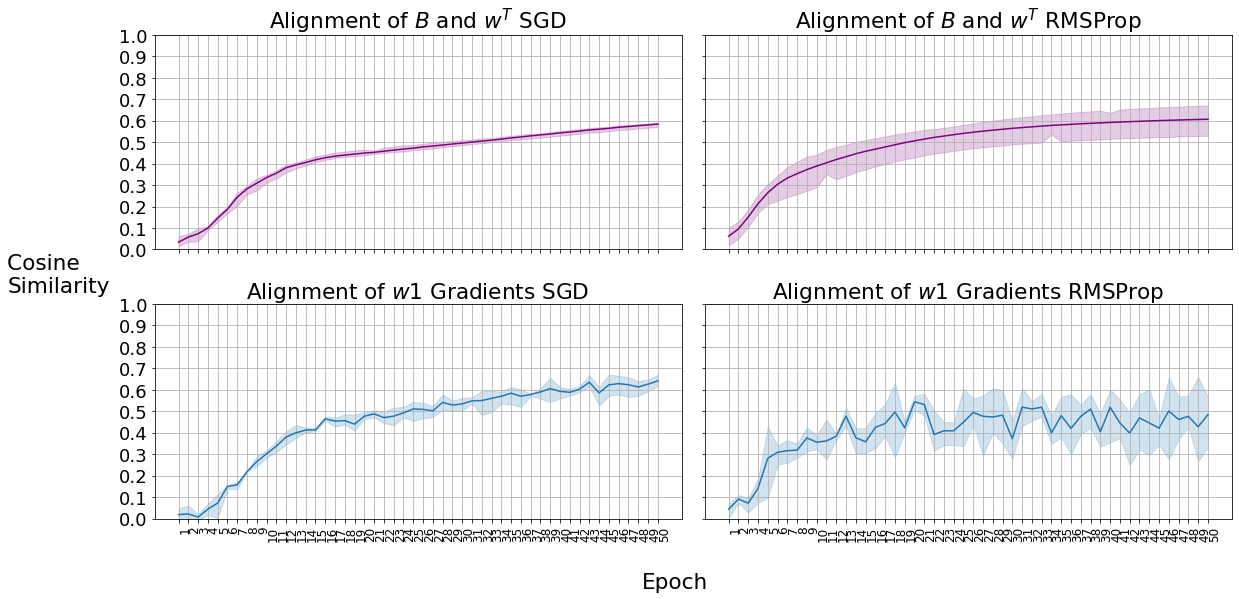
\includegraphics[width=1\linewidth]{figures/3_k3_SGD_RMSProp_DFA_Alingment} 

}

\caption[Alignment Comparison of SGD and RMSProp]{\textbf{Alignment Comparison of SGD and RMSProp} \newline The top is the alignment of the random matrix and the transpose of the weight matrix for SGD and RMSProp. The bottom is the alignment of the gradients of $w_1$ concerning loss for SGD and RMSProp. Both plots are trained on the MNIST-Parity task for the case $k=3$ for $50$ epochs.}\label{fig:Alignment}
\end{figure}

\noindent In figure \ref{fig:Alignment}, we can observe the alignment measures of SGD and RMSProp. It is interesting to point out that SGD has better alignment during the later training steps than RMSProp. From the results of the previous experiments, we know that RMSProp performed better than SGD on this task. Given that, for having better performance, alignment is not always required. On the other hand, at the beginning of the training, RMSProp aligns faster than SGD. Therefore, we can say that there is a faster alignment with adaptive methods at the beginning that prevents DFA from losing time at first epoch numbers, but later DFA finds other paths to find the minimum that is different from BP. These outcomes are parallel to results of \cite{refinetti2021align}, it was stated that DFA first aligns with BP, and later it sacrifices from this alignment to find better paths to the minimum. Apparently, this phenomenon happens quicker with adaptive methods than plain SGD.\\
\noindent One of the exciting questions that are not directly related to the predictive power of the algorithms: do the networks learn the digits individually when we train them for the MNIST-Parity task and make the necessary processes (summation, division as humans), if not what type of information does it capture? We can answer this question by observing the hidden representation of the digits. If the network learns the digits well, we need to observe a good separation like the standard MNIST task (classifying hand digits). For this purpose, hidden representations of the digits from the networks trained with BP and DFA are plotted in two-dimensional space by using t-SNE using the implementation of sklearn \cite{scikit-learn}.\\
The hidden representation of a single image in the \(k=3\) case is obtained in the following way; we know that after we flatten the images, particular parts of each image are multiplied by corresponding parts of the weight matrix. Getting these parts and performing multiplication for each digit will reveal the hidden representation of the individual digit trained in the \(k=3\) case. Process is visualized in figure \ref{fig:HiddenRepProcess}. After extracting the pixels of each image and the corresponding weights, we end up with the following matrix multiplication: \([\text{Batch Size} \times 784] [784 \space \times \space \text{Hidden Layer}]\) where \(784\) is \(28 \times 28\) and \(28\) is the pixel size of a single digit. With this matrix multiplication, we have the hidden representation of each image.

\begin{figure}

{\centering 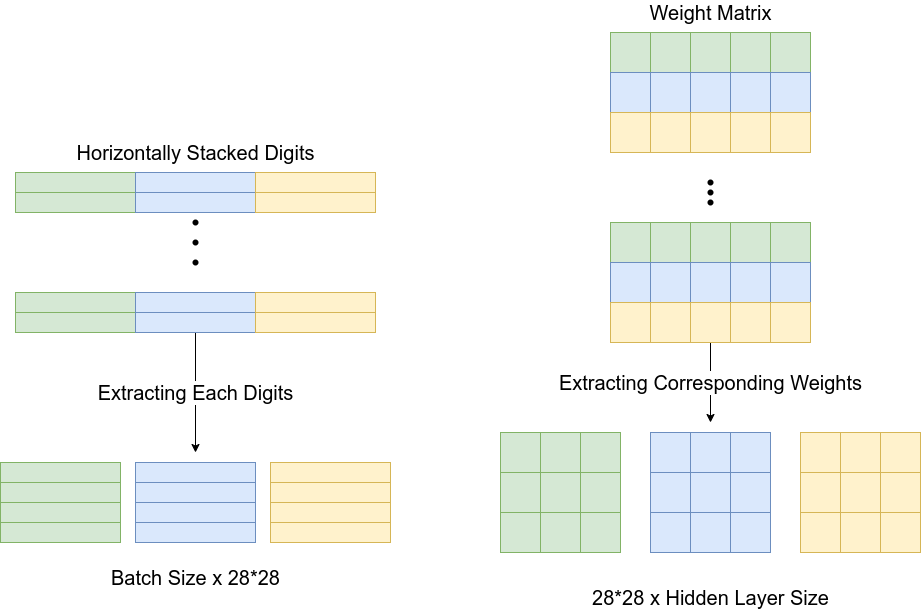
\includegraphics[width=1\linewidth]{figures/3_hidden_rep_process} 

}

\caption[Process of Extracting the Hidden Representation of Single Digit]{\textbf{Process of Extracting the Hidden Representation of Single Digit} \newline After extracting the digits and the corresponding weights, the matrix multiplication (same color) for each digit is performed separately ($28$ is the pixel size of a single digit); by doing so, we have the hidden representation of a single image from the network trained for parities of the sum of three digits.}\label{fig:HiddenRepProcess}
\end{figure}

\noindent After performing the matrix multiplication, the rest is visualizing these hidden representations by using the t-SNE. Since the t-SNE is computationally expensive, only 7500 random samples are plotted from the dataset. In figure \ref{fig:tSNEBPDFA} we can observe the results in two dimensions and say that the networks do not capture the information about the digits individually when they are trained for parities of the sum of three digits. They learn different properties of the data, not the digits individually. However, for the same purpose, transfer learning can be implemented to test if these networks trained for the parity problem can classify the digits accurately. Transfer learning is a method that involves storing the information gained while solving a problem and using this information on a different, but related problem \cite{DBLP:journals/corr/JhaS15}. Also, the same experiment can be performed for deeper networks. Maybe deeper representations of the parities might contain information about the digits individually. These experiments are left for future studies. On the other hand, it is not surprising that BP and DFA capture very similar information from the MNIST-Parity dataset.

\begin{figure}

{\centering 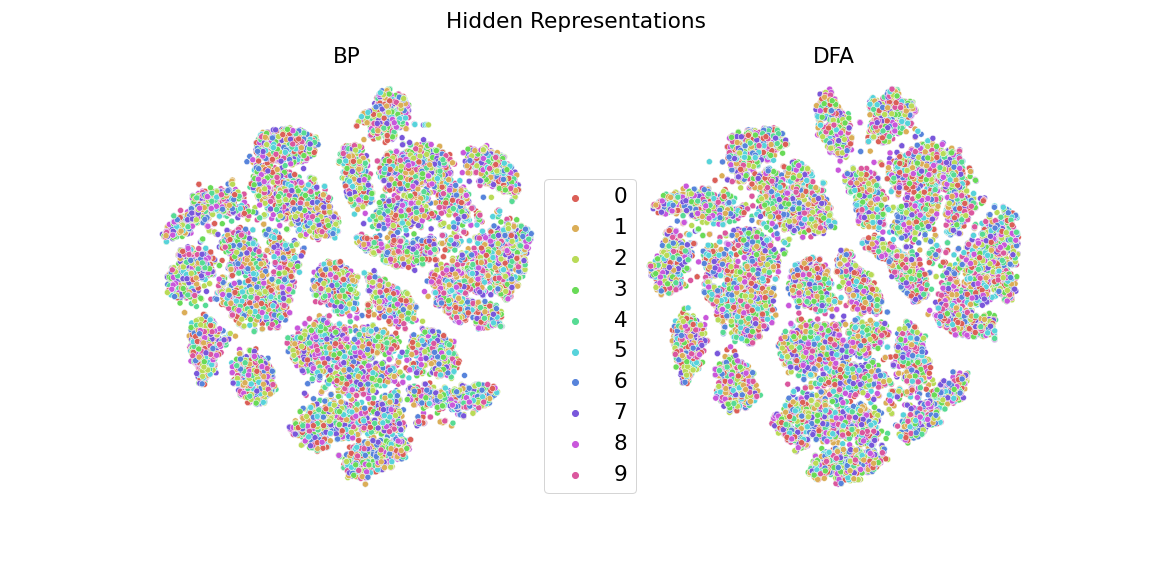
\includegraphics[width=1\linewidth]{figures/3_tsne_BPDFA} 

}

\caption[Hidden Representation of Digits in BP and DFA]{\textbf{Hidden Representation of Digits in BP and DFA} \newline Hidden representations of images are visualized with their labels for BP and DFA. The process of acquiring these representations is explained in \ref{fig:HiddenRepProcess}.}\label{fig:tSNEBPDFA}
\end{figure}

\hypertarget{synthetic-data-experiments}{%
\section{Synthetic Data Experiments}\label{synthetic-data-experiments}}

After having the previous experiment result and current experiments details for synthetic data, we can test the DFA on the number of dimensions plots with the test error to compare with BP. Most of the parameters are the same as MNIST-Parity experiments. The only difference is the learning rate. The learning rate is set to \(0.5\) without hyperparameter tuning for all methods. They are performed with three repetitions and plotted with their \(95\%\) confidence interval.

\begin{figure}

{\centering 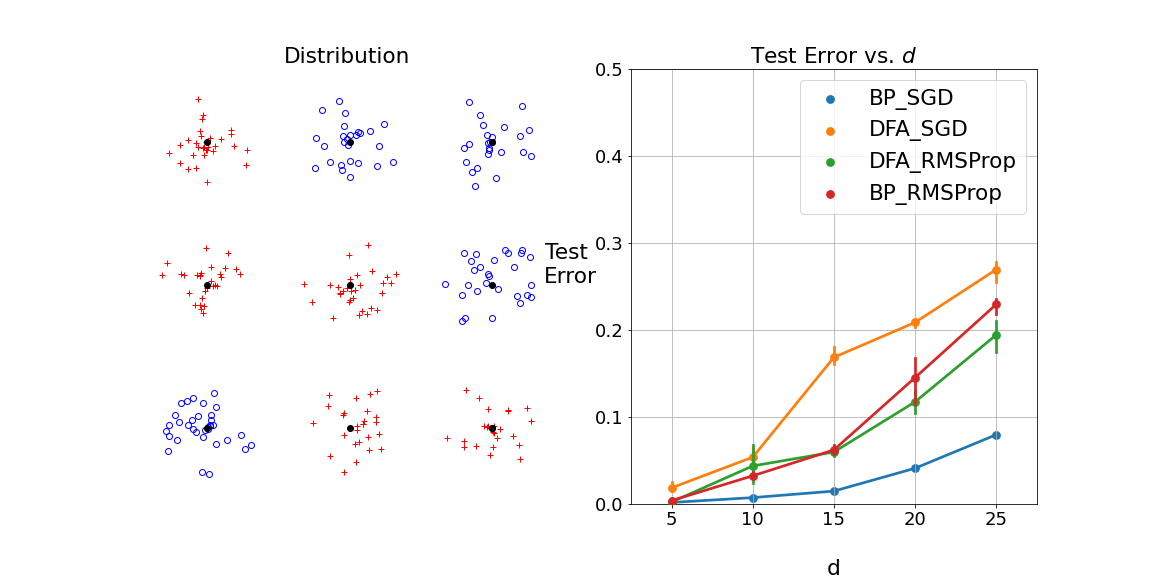
\includegraphics[width=1\linewidth]{figures/3_syntheticData_adaptive} 

}

\caption[BP and DFA on Synthetic Data Problem]{\textbf{BP and DFA on Synthetic Data Problem} \newline On the left, the input distribution of the two first dimensions is used for the experiment. On the right, test error of BP and DFA with SGD and RMSProp as a function of the number of dimensions ($d$) where the number of inputs is $256$ ($n = 256$).}\label{fig:DFARandom}
\end{figure}

\noindent Before interpreting the results, it is essential to mention that experiment results will be drastically different if the input distribution has changed. We have chosen a distribution that shows the difference among the algorithms well. It would be more convenient to run for different datasets with more repetition and plot the average. We left this for future considerations.
\noindent We can observe the results in \ref{fig:DFARandom}. DFA performs better than the lazy method. However, BP with SGD outperforms the DFA. Since it is natural to try adaptive methods to hope for an improvement, as we experienced for the parity experiments, we used RMSProp on the same problem both for BP and DFA. It again increases the predictive power of DFA, but it is still behind the BP with SGD. It is also interesting that BP with RMSprop did not perform better than plain BP with SGD. It might be due to the implicit bias of adaptive methods (while fitting the data, the adaptive methods might choose global minima of the training loss with suboptimal generalization error), or sometimes adaptive methods can have unexpected problems in simple settings, such as convex problems (this distribution might be another example of this) \cite{reddi2019convergence}. Understanding why adaptive methods affect BP and DFA differently is an intriguing avenue for further works.\\
\noindent Moreover, it is promising that DFA improves with one adaptive method for another challenging learning problem. We have to specify that, It would be intriguing to observe well-tuned DFA with different adaptive methods on the same problem; this is again left for future investigations.\\

\noindent \textbf{Highlights}\\
With the synthetic data experiment, we conclude the experiments. We started with testing the predictive power of DFA on the MNIST-Parity task. Then, we visualized the alignment of the random matrix and the transpose of the weights. After that, we tried to improve the performance of DFA by trying different types of random matrices, and we used adaptive methods. We discovered that with the help of adaptive methods, DFA could perform as well as BP within the same epoch numbers. For investigating why adaptive methods help DFA more than BP, we compared the alignments of SGD and RMSProp for DFA. We concluded that better alignment does not always mean better performance. Then, we visualized the hidden representations of the digits from the network trained for the MNIST-Parity task. We observed that networks do not capture information about the digits individually. Lastly, we performed the synthetic data experiment using a fixed distribution. We plotted the final test error of BP and DFA, both with SGD and RMSProp as the function of the number of dimensions. Once again, we noticed that adaptive methods boost the performance of DFA. We left some further experiments of synthetic data for future studies.

\hypertarget{conc}{%
\chapter*{Conclusion}\label{conc}}
\addcontentsline{toc}{chapter}{Conclusion}

This research aimed to compare DFA with BP on the particular learning problems that proved the superiority of the BP over the linear methods. Moreover, we tried to improve their predictive power on these learning problems. In doing so, we hoped to understand their learning dynamics better.\\
Thanks to the error propagation mechanism of DFA, it proposes a more biologically plausible algorithm than BP. However, the performance is still an enormous part of the success of the algorithms. Furthermore, based on the theoretical foundations of the algorithms that we presented in chapter \ref{chap:chapter_1}, it was expected to experience performance lag for DFA behind BP. For validating this empirically, we used a set of learning problems that are explained in chapter \ref{chap:chapter_2}. In previous studies, these problems proved the dominance of the BP over the lazy methods. After reproducing the previous experiments from these studies, we tested DFA on the same problems. Our expectations were validated with the initial results. These results are demonstrated in chapter \ref{chap:chapter_3} among other experiments. Although DFA performed better than the linear methods, there was a performance gap between plain DFA and BP without any intervention. Then, we tried to close this gap by performing a few modifications either on the training algorithm or the optimization process. Even though these modifications did not constantly improve the performance, we acquired a deeper understanding of algorithms' learning behaviors. They opened the gate of correct interventions to close the gaps. Finally, these interventions yield that using adaptive optimizers, DFA could perform equal or close to BP's predictive performance on the particular learning problems that the lazy methods notoriously failed or did not perform well.\\
Although we performed various experiments that investigate the performance and learning behaviors of the algorithms, there are still too many aspects that need to be investigated further. For instance, we used architectures with only a hidden layer, and layer size was \(512\); so the network's depth and the layer's width are not investigated further. Different activation functions are not tested apart from reLU. It would be intriguing to observe the behavior of DFA with these aspects. Also, one of the experiments that analyze the hidden representation of the digits in the parity learning problem can be extended. For instance, transfer learning can be implemented to test if networks trained for the parity problem can classify the digits accurately. In other words, the network trained for the parity learning problem can be tested to classify the digits. Although these hidden representations demonstrated the opposite, one might find a trace of learning of the digits. In addition to these propositions, the learning problems can constantly be enriched, and new challenging problems can be considered with DFA. Also, different alternative algorithms can be tested on these challenging problems. Furthermore, all the theoretical and empirical aspects of the learning problems we use were not analyzed. For instance, we used a fixed distribution for the synthetic data problem. One might want to use more distributions and observe the average of the predictive powers of the algorithms. Moreover, for the synthetic data experiment, we observed that adaptive methods have a different effect on DFA and BP. Understanding the reason behind this is an attractive path to pursue. All these kinds of further experiments are left for future studies.\\
BP is the touchstone for training neural networks. Although the community demonstrated gigantic advancements for optimization methods or architecture types of the networks, BP is still around for decades, and the algorithm's success is indisputable. It is vital to point out that the advancement of BP did not happen in one day. DFA and other alternative algorithms bring a new perspective on the training phase of the networks. With this, we can remove some of the restrictions enforced by BP, such as biological implausibility, lack of parallelism, et cetera. We believe that testing the different aspects of the alternative algorithms and comparing them with BP would contribute a lot to the success of deep learning. These studies might spawn more robust training algorithms which obey the biological plausibility, and they might even train faster with a performance close or equal to BP.~

\startappendices

\hypertarget{chap:appendix_a}{%
\chapter{Backpropagation with Binary Cross-Entropy}\label{chap:appendix_a}}

Following calculations are heavily inspired from these notes\footnote{\url{https://www.ics.uci.edu/~pjsadows/notes.pdf}}. The notation and the general structure might differ, but the idea is the same.\\
Let us consider a simple binary classification task. It is common to use a network with a single logistic output with the binary cross-entropy loss function and for the sake of simplicity, let us assume that there is only one hidden layer.
\[
\begin{aligned}
BCE=-\sum_{i=1}^{n o u t}\left(y_i \log \left(\hat{y}_i \right)+\left(1-y_i\right) \log \left(1-\hat{y}_i\right)\right)
\end{aligned}
\]
\noindent Where \(y\) is the ground truth and \(\hat{y}\) is the output of the network. After having the loss function, let us continue with the forward pass.

\[
\begin{aligned} 
a_{k} &= h_{k-1} w_{k} + b_k \\
h_k &= f(a_{k})
\end{aligned}
\]
\noindent Where, \(w_k\) is the weight, \(b_{k}\) is the bias term, \(h_k\) is the output of the layer (which means that \(h_0 = X\) and \(h_2 = \hat{y}\)) and f is the non linear function. Please note that for last layer logistic function is used whereas for hidden layer reLU is used as non linear functions.\\
We can compute the derivative of the weights by using the chain rule.

\[
\begin{aligned} 
\frac{\partial BCE}{\partial w_{2}}=\frac{\partial BCE}{\partial \hat{y}} \frac{\partial \hat{y}}{\partial a_{2}} \frac{\partial a_{2}}{\partial w_{2}}
\end{aligned}
\]
\noindent Computing each factor in the term, we have:
\[
\begin{aligned}
\frac{\partial BCE}{\partial \hat{y}} &=\frac{-y}{\hat{y}}+\frac{1-y}{1-\hat{y}} \\
&=\frac{\hat{y}-y}{\hat{y}\left(1-\hat{y}\right)} \\
\frac{\partial \hat{y}}{\partial a_{2}} &=\hat{y}\left(1-\hat{y}\right) \\
\frac{\partial a_{2}}{\partial w_{2}} &=h_{1}^T
\end{aligned}
\]
This expression gives us:
\[
\frac{\partial BCE}{\partial w_{2}}=h_{1}^T\left(\hat{y}-y\right)
\]
We can calculate the derivative of the \(w_1\) concerning loss function as the following:

\[
\begin{aligned} 
\frac{\partial BCE}{\partial w_{1}}=\frac{\partial BCE}{\partial h_1} \frac{\partial h_1}{\partial a_{1}} \frac{\partial a_{1}}{\partial w_{1}}
\end{aligned}
\]
Compute each factor in the term again, we have:

\[
\begin{aligned}
\frac{\partial BCE}{\partial h_1} &= \frac{\partial BCE}{\partial \hat{y}} \frac{\partial \hat{y}}{\partial a_{2}} \frac{\partial a_{2}}{\partial h_{1}}  \\
&= \left(\hat{y}-y\right) w_{2}^T \\
\frac{\partial h_1}{\partial a_{1}} &=f'(a_1) \\
\frac{\partial a_{1}}{\partial h_{1}} &=X^T
\end{aligned}
\]
This expression gives us:
\[
\begin{aligned}
\frac{\partial BCE}{\partial w_{1}}= \left(X\right)^T\left(\hat{y}-y\right)\left(w_{2}^T\right) \odot f'(a_1)
\end{aligned}
\]
Where \(\odot\) is element-wise multiplication, similarly, bias terms can be calculated by following:

\[
\begin{aligned} 
\frac{\partial BCE}{\partial b_{2}}&=\frac{\partial BCE}{\partial \hat{y}} \frac{\partial \hat{y}}{\partial a_{2}} \frac{\partial a_{2}}{\partial b_{2}} \\
&= \left(\hat{y}-y\right)
\end{aligned}
\]

\[
\begin{aligned} 
\frac{\partial BCE}{\partial b_{1}}&=\frac{\partial BCE}{\partial h_1} \frac{\partial h_1}{\partial a_{1}} \frac{\partial a_{1}}{\partial b_{1}} \\
&= \left(\hat{y}-y\right)\left(w_{2}^T\right) \odot f'(a_1)
\end{aligned}
\]
After having all these results, we can update the parameters (weights and biases) using gradient descent and its variants.

\hypertarget{direct-feedback-alignment-with-various-learning-rates}{%
\chapter{Direct Feedback Alignment with Various Learning Rates}\label{direct-feedback-alignment-with-various-learning-rates}}

We have mentioned that DFA is highly sensitive to the learning rate throughout the experiments. We want to support this argument with some plots. For this purpose, we plotted validation accuracy for each learning rate value during the hyperparameter tuning of different random matrices. The networks are trained for the MNIST-Parity task for the case \(k=3\) with SGD up to \(20\) epochs.

\begin{figure}

{\centering 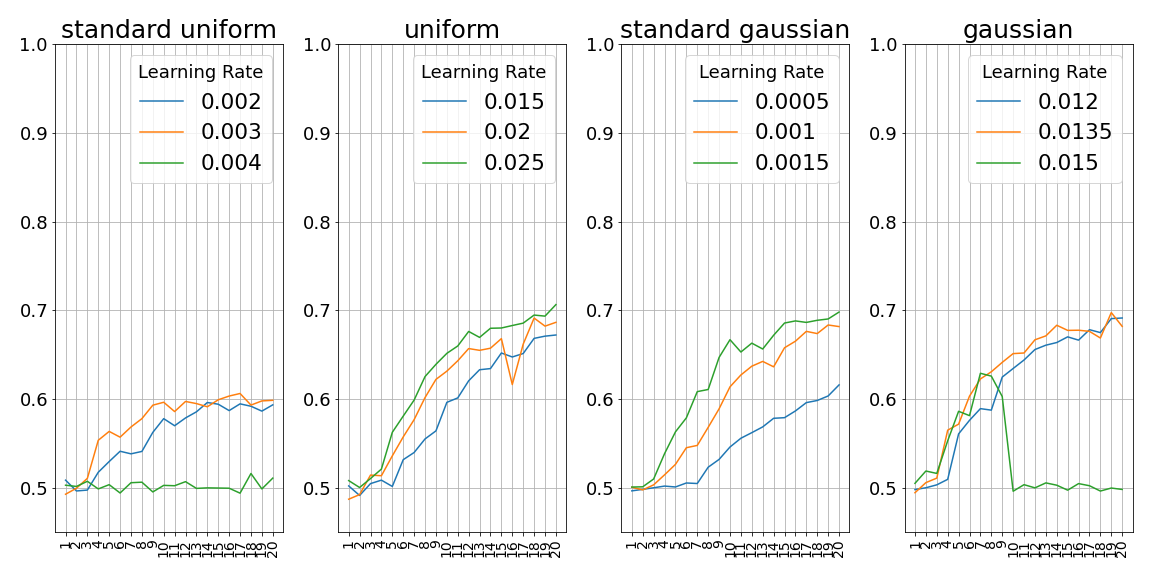
\includegraphics[width=1\linewidth]{figures/B_k3_SGD_DFA_BInitsWDifferentlrs} 

}

\caption[Various Random Matrix Initialization with Different Learning Rates]{\textbf{Various Random Matrix Initialization with Different Learning Rates} \newline The predictive power of DFA with various random matrix initializations on MNIST-Parity task. The model tries to predict the parities of the sum of three digits and it is trained with SGD. The random matrices are initialized as the following: $\text{standard uniform} \sim U(0,1)$, $\text{uniform} \sim U(-a,+a)$, $\text{standard gaussian} \sim \mathcal{N}\left(0, 1\right)$ and $\text{gaussian} \sim \mathcal{N}\left(a, a \right)$ where $a= \frac{1}{\sqrt{input dim}}$.}\label{fig:BinitWDifferentLR}
\end{figure}

\noindent The result can be observed in figure \ref{fig:BinitWDifferentLR}. We can see that some high learning rate values do not even provide performance beyond a random guess as in the standard uniform random matrix. For the gaussian random matrix, if we have a high learning rate, we can observe increasing accuracy and a rapid decrease later. These patterns may also happen with other initializations, even with adaptive methods. We suggest decreasing the learning rate to have more stable patterns in these cases.\\
We performed the same process for adaptive methods. Again, the networks are trained for the MNIST-Parity task for the case \(k=3\) up to \(20\) epochs. The results for the adaptive methods can be observed in figure \ref{fig:AdaptiveWDifferentLR}.

\begin{figure}

{\centering 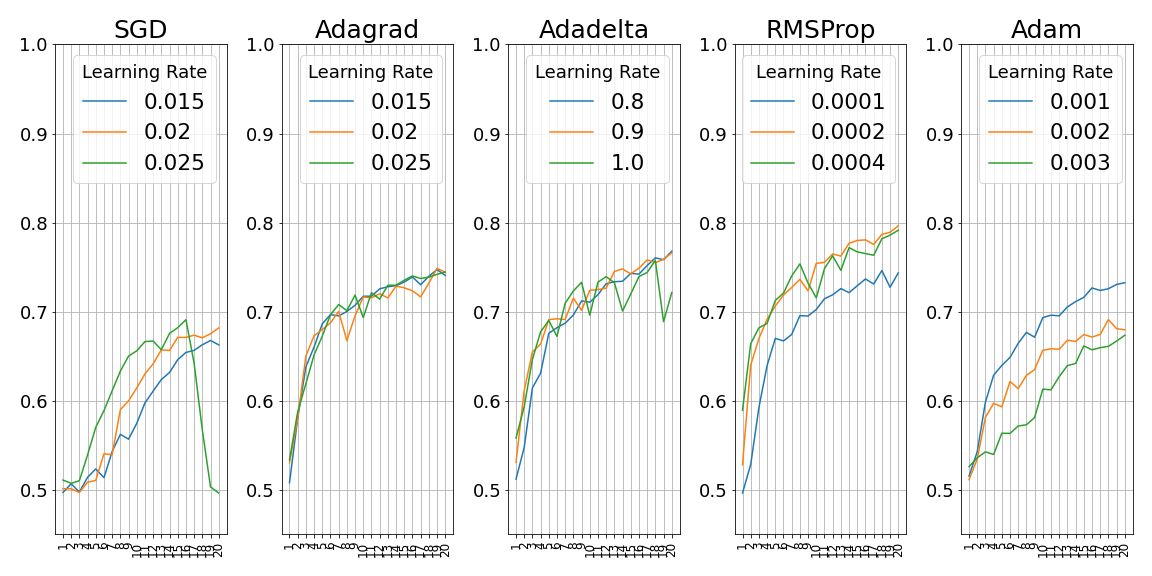
\includegraphics[width=1\linewidth]{figures/B_k3_All_DFA_optimsWDifferentlrs} 

}

\caption[Various Adaptive Methods with Different Learning Rates]{\textbf{Various Adaptive Methods with Different Learning Rates} \newline The predictive power of DFA is presented with adaptive methods on the MNIST-Parity task. Random matrices are initialized uniformly. The model tries to predict the parities of the sum of three digits with different learning rates.}\label{fig:AdaptiveWDifferentLR}
\end{figure}

\noindent We can see that adaptive methods are more robust than plain SGD. However, similar to the previous plot, it is possible to observe comparable patterns. Indeed, Adadelta draws a zig-zag pattern with a high learning rate.

\hypertarget{reproducibility}{%
\chapter{Reproducibility}\label{reproducibility}}

For reproducing the experiment results, please refer to this Github repository\footnote{\url{https://github.com/demirbilek95/Dynamics-of-Learning}}. It contains all the codes that are used to have the experiment results. It also includes the requirements to run the code. However, due to the stochastic behavior of the neural networks and the data, results will not be precisely the same. Nevertheless, it must be very close to the presented ones on average. Stochastic behaviors can be explained as the following: The neural network weights and the random matrix (for DFA) are sampled from a uniform distribution so that each instance will be slightly different. Given the parameter \(k\), the parity data is sampled uniformly from the MNIST dataset. In addition to this, it is recreated for each epoch, so we had a different dataset at every iteration. DFA is extremely sensitive to the learning rate, so occasionally, overfitting might be observed, meaning that validation accuracy might decrease instantly in the middle of training. For overcoming this issue, we suggest decreasing the learning rate. Although we used a fixed distribution, the synthetic data also follows stochastic behavior. The labels of the clusters are assigned randomly, and the cluster samples are distributed from a uniform distribution (it is explained detailly in \ref{chap:chapter_2}). The distribution of the first two dimensions is plotted with experiments. Other distributions would give different results. Hyperparameters used in the experiments can be found in the Github repository, and the process of how they are tuned or which value they are set is explained in the related chapters.\\
Lastly, a local computer is used for all the experiments, and all the experiments are performed on GPU (Nvidia GTX 960M).


%%%%% REFERENCES
\setlength{\baselineskip}{0pt} % JEM: Single-space References

{\renewcommand*\MakeUppercase[1]{#1}%
\printbibliography[heading=bibintoc,title={\bibtitle}]}


\end{document}
